\documentclass[12pt]{article}
\usepackage[utf8]{inputenc}
\usepackage{bm}                                     % bold in math env
\usepackage{import}                                 % import package
\usepackage{colortbl}
\usepackage[table]{xcolor}
\usepackage{url}
\usepackage{graphicx}
\usepackage{parskip}
\usepackage{fancyhdr}
\usepackage{vmargin}
\usepackage{geometry}
\usepackage{caption}
\usepackage{subcaption}
\usepackage{tcolorbox}                              % Beautiful box 
\usepackage{hyperref}
\usepackage{amsfonts,amsmath,amssymb,amsthm}        % all the math in one 
\usepackage{amsfonts}
\usepackage{tikz}                                   % drawing package
\usepackage[acronym, toc]{glossaries}               % Module for glossary
\usepackage{acronym}                                % Module for acronyms
\usepackage{xargs}                                  % more than one args in cmd
\usepackage{mathrsfs}                               % Cursive font
\usepackage{afterpage}                              % https://ctan.org/pkg/afterpage
\usepackage{float}                                  % Position of float
\usepackage{subfig}
\usepackage{makecell}                               % \Xhline{NUM\arrayrulewidth}


% https://tex.stackexchange.com/questions/20575/attractive-boxed-equations
\usepackage{empheq}                         

% { ..
% ..TODO REMOVE WHEN READY
\usepackage{lipsum}                                 
\usepackage[nottoc]{tocbibind}
\usepackage[firstpage]{draftwatermark}
\SetWatermarkText{DRAFT}
\SetWatermarkScale{4}
\SetWatermarkColor[rgb]{0.7,0.1,0.2}
\usepackage[pdftex,dvipsnames]{xcolor}  % Coloured text etc.
\usepackage[colorinlistoftodos,prependcaption,textsize=tiny]{todonotes}
\newcommandx{\unsure}[2][1=]{\todo[linecolor=red,backgroundcolor=red!25,bordercolor=red,#1]{#2}}
\newcommandx{\change}[2][1=]{\todo[linecolor=blue,backgroundcolor=blue!25,bordercolor=blue,#1]{#2}}
\newcommandx{\info}[2][1=]{\todo[linecolor=OliveGreen,backgroundcolor=OliveGreen!25,bordercolor=OliveGreen,#1]{#2}}
\newcommandx{\improvement}[2][1=]{\todo[linecolor=Plum,backgroundcolor=Plum!25,bordercolor=Plum,#1]{#2}}
\newcommandx{\thiswillnotshow}[2][1=]{\todo[disable,#1]{#2}}
% }

\setlength{\parindent}{0pt}     % Annule indentation automatique
\setlength{\parskip}{2ex}       % Saut de ligne

\title{Contrôle d'un agent via apprentissage par renforcement}
\author{Makdoud Nizam}
\date{\today}

% { -- Esthétique

\makeatletter
\let\thetitle\@title
\let\theauthor\@author
\let\thedate\@date
\makeatother

\pagestyle{fancy}
\fancyhf{}
\rhead{\theauthor}
\lhead{\thetitle}
\cfoot{\thepage}

% }


%% -- Redefinition
\renewcommand{\contentsname}{Table des matières} 
\renewcommand*\listfigurename{Liste des figures}
\renewcommand*{\acronymname}{Abréviations}
\renewcommand{\glossaryname}{Glossaire}

\makenoidxglossaries

% -- simple test

\newglossaryentry{A3C}
{
    name=A3C,
    description={Acronyme pour  Asynchronous Actor-Critic Agents qui est l'algorithme qui servira de base pour le contrôle de notre agent.}
}


\newglossaryentry{IA}
{
    name=IA,
    description={Acronyme d'intelligence artificielle, cela désigne un ensemble de technologie visant à un apprentissage automatique. En particuliers, pendant ce stage, nous explorerons des sous-parties de l'intelligence artificielle qui sont l'apprentissage profond et l'apprentisage par renforcement.}
}


\newglossaryentry{API}
{
    name=API,
    description={En anglais: \emph{Application program interface}, c'est un ensemble de protocoles, ou de contrats spécifiant le fonctionnant d'un programme. Dans le cas de ce rapport, cela correspond à un contrat entre l'application client et serveur (SE-STAR)}
}

\newglossaryentry{RL}
{
    name=RL,
    description={RL est l'acronyme de reinforcement learning qui en francais se traduit par apprentissage par renforcement.}
}


\newglossaryentry{GPU}
{
    name=GPU,
    description={En anglais: \emph{Graphics Processing Unit}, est un composant normalement utilisé dans la gestion des graphismes qui permet d'effectuer des calcules hautement parallèlisable de façon extrêmement rapide}
}

\newglossaryentry{PAAC}
{
    name=PAAC,
    description={Référence à une méthode en apprentissage par renforcement nommée \emph{Efficient Parallel Methods for Deep Reinforcement Learning }\cite{2017arXiv170504862C}. Elle se repose sur la même stratégie que l'A3C en utilisant une architecture synchrone permettant l'utilisation du GPU} 
}

\newglossaryentry{Wine}
{
    name=Wine,
    description={En anglais: \emph{Wine Is Not an Emulator}, est une application permettant l'utilisation d'application Windows sous Linux. Son nom vient du faite que de nombreuses personnes pensent a tort que Wine est un 'emulateur de Windows' or Wine a réimplémenté l'ensemble des appels systèmes dans le user space linux permettant à l'utilisateur de faire fonctionner une application Windows sous une distriubtion Linux}
}


\newglossaryentry{framework}
{
    name=framework,
    description={Un framework est un logiciel proposant une architecture unifiée répondant à une problématique. Dans ce rapport, on pourra parler de framework de deep learning qui sont des outils proposant une API dans la réalisation de nos algorithmes.}
}

\newacronym{gcd}{GCD}{Greatest Common Divisor}




% --------------------------------------------------------------------------
%%                                  BEGIN
% --------------------------------------------------------------------------

\begin{document}

\pagenumbering{roman}

% ============================================================
% Mise en page du titre
% cfhttps://www.overleaf.com/10351077tkgybggqnnsh#/38448375/
% ============================================================
\setmarginsrb{3 cm}{2.5 cm}{3 cm}{0 cm}{.5 cm}{1.5 cm}{0 cm}{0 cm} % Quick Hack 

\begin{titlepage}
	\centering
    
\includegraphics[scale = 0.70]{./assets/ensem}\\[.75 cm]	% University Logo
    \textsc{\large École National Supérieur d'électricité et de Mécanique}\\[1.7 cm]	% University Name

	\rule{\linewidth}{0.5 mm} \\[.8 cm]
	{ \huge \bfseries \thetitle}\\[.65cm]
	\rule{\linewidth}{0.5 mm} \\[1.cm]
	
	\begin{minipage}{0.4\textwidth}
		\begin{flushleft} \large
			\emph{Auteur:}\\
			\theauthor
			\end{flushleft}
			\end{minipage}~
			\begin{minipage}{0.4\textwidth}
			\begin{flushright} \large
			\emph{Tuteur:} \\
			A\\
			B\\
			C									
		\end{flushright}
	\end{minipage}\\[1.3 cm]
	
	\today\\[1. cm]

    \begin{minipage}[c]{0.45\linewidth}
        \hspace{-2cm}
\includegraphics[width=1.4\linewidth]{./assets/thales}
    \end{minipage} \hfill
    \begin{minipage}[c]{0.45\linewidth}
        
\includegraphics[width=1.4\linewidth]{./assets/inria}
    \end{minipage}

\end{titlepage}

\newpage

% =================================
% MACRO 
% =================================

\newcommand{\norm}[1]{\left\lVert\: #1 \:\right\rVert}
\newcommand\bsum{\mathlarger{\sum}}          % big summation
\newcommand\discountedReward{\sum_{k=0}^{\infty} \gamma^kR_{t+k+1}}
\newcommand\valueFunction{\mathbb{E_\pi}\bigg(\sum_{k=0}^{\infty} \gamma^kR_{t+k+1}  \:\bigg\vert\: s_t=s \bigg)}
\newcommand\QFunction{\mathbb{E_\pi}\bigg(\sum_{k=0}^{\infty} \gamma^kR_{t+k+1}  \:\bigg\vert\: s_t=s, a_t=a \bigg)}

% Policy with color to highlight the conditional probability (policy color -> policyc)
\newcommand{\policyc}[1]{
    \textcolor{#1}{
        \underbrace{\pi(x\:,\:a)}_{p\:(a \:\vert\: s)}
    }
}

\newcommand{\dynamicsc}[1]{
    \textcolor{#1}{
        \overbrace{T(s',r , s, a)}^{p(s',r \vert s, a)}
    }
}


% =================================
% Résumé - Remerciement
% =================================


% Just the default setting 
\setmarginsrb{3 cm}{2.5 cm}{3 cm}{2.5 cm}{1 cm}{1.5 cm}{1 cm}{1.5 cm}
\thispagestyle{empty}

\section*{Remerciements}
\bigskip
Je tiens à remercier chaleureusement toutes les personnes qui m'ont accompagnées durant ce stage pour faire de ces six mois une expérience  profitable sur le plan professionnel et agréable sur le plan personnel.


\noindent Tout d'abord, je remercie Jérome Kodjabachian, Marc Shoenauer et Christophe Meyer pour m'avoir donné l'opportunité d'effectuer ce stage, de m'avoir conseillé et  permis de m'épanouir durant ces six mois.


\noindent Je remercie également Alexandre kazmierowski pour son soutien, ses conseils assidus et sa disponibilité sans laquelle je n'aurais pas pu avancer sur certains points de ce stage.   


\noindent Enfin, je tiens à remercier l'ensemble de l'équipe AS&BSIM, pour sa sympathie et sa disponibilité.
\newpage
\thispagestyle{empty}
\section*{Abstract}
\bigskip

Artificial intelligence is a growing field which aims is to improve task automation. Through this internship, a subfield of artificial intelligence named reinforcement learning has been explored.

Reinforcement learning deals with issues governed by a set of rewards. For example, the classical problem in reinforcement learning is the control of agent through one place to another. The agent receives a reward when it arrives to the final place.  The goal of our control is to find the optimal sequence of actions that maximises the cumulated rewards, which is, for our example, to reach to goal within the shortest time.

THALES is involved in the infrastructure security design, and aims to ensure the security of infrastructuresby created plans to scenarios generated by SE-STAR. 
SE-STAR is a simulation capable of created mutltiple scenarios which may involve a large number of agents. SE-STAR uses internals drives (like hunger, fear, stress ...) to control the mass of agents but these internal drives has to be carefully design to accomplish a scenario (like a fight in a gare).

We choose another way of controlling agents that uses only rewards to automatically find the optimal behaviour that correspond to a given scenario.
Notably, we have worked on the control of an agent in a simulated environnement created by the thales' internal biomimetic simulation SE-STAR.

We will propose mutltiple architectures and reinforcement learning algorithms to allow an agent to move in its simulated environnement by its own internal motivation to find our specified goal. The novelty of this approch is to find a policy with a weakly informative input like the partial vision of the agent which banned the use of other traditionnal control algorithms. 

Non-exhaustively, the internship has been divided in five periods:

\begin{itemize}
    \item Bibliographic and litterature search.
    \item Application of main algorithms on simple environnements.
    \item Development of reinforcement learning algorithms on 2D and 3D environnements used by researchers to benchmark their controllers. 
    \item Design of a wrapper around the simulation SE-STAR to support the use of our external algorithm.
    \item Research of algorithms based on intrinsic motivations (or curiosity) to help the agent to find the optimal policy in difficult 3D environnements like those created by SE-STAR. 
\end{itemize} 

\newpage


\section*{Résumé}
\bigskip

L'apprentissage automatique est un domaine subissant actuellement une forte expansion, permettant une automatisation de nombreuses tâches. A travers ce stage, nous avons exploré une sous partie de l'apprentissage automatique qui se nomme l'apprentissage par renforcement profond. 

Ce domaine vise à résoudre des problèmes qui sont régis par des récompenses. Par exemple, nous pouvons imaginer le problème d'un agent ayant pour but d'aller d'un point A à un point B, une récompense serait donné à l'agent dès qu'il attendra le point B. Notre objectif sera de trouver la politique optimale de l'agent pour maximiser la quantité de récompense reçue. Dans notre exemple, l'agent aura à apprendre la séquence d'actions qui permettra d'aller jusqu'au point B, et ainsi d'obtenir le maximum de récompenses. En particulier, nous travaillerons à l'aide d'un logiciel de simulation bio-inspiré qui se nomme SE-STAR. 

Nous proposerons une architecture et des algorithmes d'apprentissage par renforcement permettant à un agent de se déplacer dans l'environnement simulé à la recherche de la sortie de façon non supervisée. 

De manière non exhaustive, nous pouvons définir ce stage en cinq périodes: 
\begin{itemize}
    \item Découverte et recherche bibliographique.
    \item Application des principaux algorithmes sur des cas simples.
    \item Élaboration d'algorithmes de renforcements profonds sur des environnements 2D et 3D utilisés par les chercheurs pour comparer la performance de leurs méthodes
    \item Conception d'un outil autour de SE-STAR pour supporter les algorithmes d'apprentissage par renforcement.
    \item Recherche autour d'une solution adaptée spécifiquement à l'apprentissage par renforcement profond dans le cadre problématique des environnements labyrinthiques.
\end{itemize}

Ci dessous une représentation des grandes périodes pendant ce stage:

\begin{center}
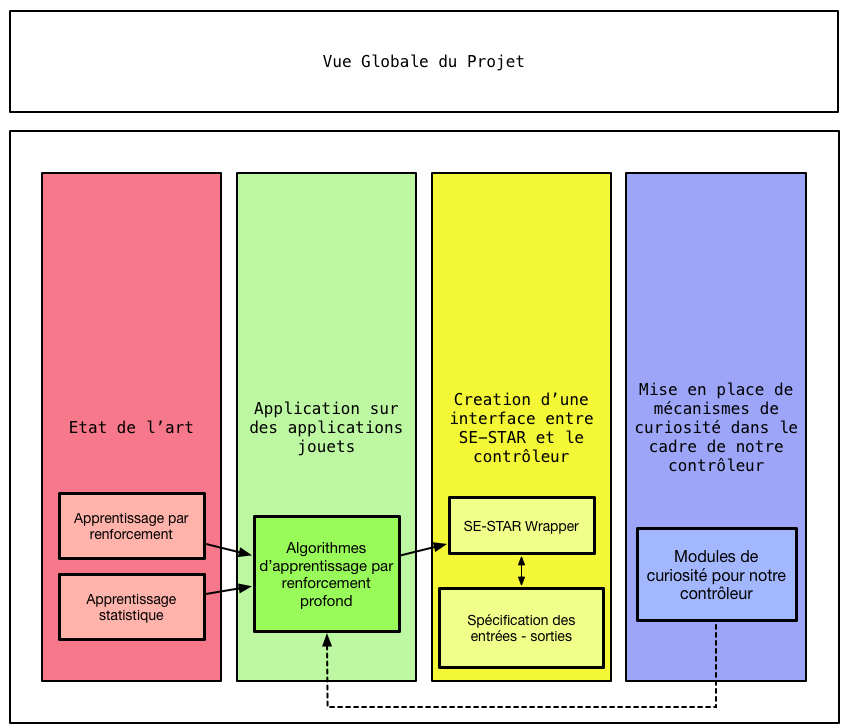
\includegraphics[scale=.5]{./assets/globale.png}
\end{center}

\newpage

% =================================
% Table des matières et autres
% =================================

\thispagestyle{empty}
\listoffigures   \newpage

\printglossary[type=\acronymtype]
\printglossary

\thispagestyle{empty}
\tableofcontents \newpage


% =================================
% Corps du rapport
% =================================

\pagenumbering{arabic}
\setcounter{page}{1}

\section{Introduction}

Dans le cadre de ma formation d'ingénieur à l'\emph{École Nationale Supérieure d'électricité et de Mécanique}, j'ai réalisé un stage du 2 février 2017 au 2 août 2017 au sein du laboratoire ThereSIS de THALES Services à Palaiseau, dans le campus de Saclay. J'ai eu l'occasion pendant ce stage d'effectuer de nombreux séjours à l'INRIA Tao pendant lesquels j'ai pu m'entretenir avec des chercheurs en apprentissage par renforcement et me tenir au courant des avancées dans le domaine de l'intelligence artificielle.

J'ai réalisé ce stage au sein de l'équipe AS&BSIM (Adaptative Systems and
Biomimetic Simulation), qui travaille principalement sur le logiciel \textbf{SE-STAR}. Il s’agit d’un environnement synthétique où évoluent de nombreux agents virtuels, chacun disposant d’un modèle cognitif. 

Dans le cadre de ces simulations, je me suis intéressé à la navigation d'un agent en utilisant l'apprentissage par renforcement profond pour contrôler l'agent dans son environnement. En particulier, la contrainte imposée sur le contrôle de l'agent est qu'en entrée du contrôleur, nous n'avions accès qu'à une image 2D d'un environnement 3D (en l'occurrence SE-STAR).



\subsection{Contexte du stage et de l'entreprise}

Le groupe THALES est une multinationale française employant 67 000 salariés
dans 56 pays. Si l’entreprise est connue auprès du grand public pour sa présence
sur le marché de la défense, elle opère aussi sur plusieurs marchés duaux (à la
fois civils et militaires) : l’aéronautique, l’espace et la sécurité, ainsi que sur le
marché civil du transport terrestre. Les problématiques de traitement et
interprétation des données ainsi que d’aide à la prise de décision sont au cœur
de l’activité du groupe. Afin de renforcer la position du groupe dans l’innovation
autour des nouvelles technologies, les activités de recherche et développement
sont au cœur de l’entreprise, représentant 20\% de ses revenus. THALES possède
un réseau international de laboratoires qui coopèrent avec des universités et des
laboratoires de recherche publics.

THALES Services est une division de THALES, dont l’activité se situe autour des
systèmes d’information et de communications sécurisés.
ThereSIS (THALES European Research for E-Government & Secured Information
Systems) est le laboratoire de recherche en systèmes d’information de THALES
Services. Il est situé sur le site de THALES Research and Technology à Palaiseau.
Les équipes en place ont pour mission de tester des technologies
innovantes, afin de déterminer si elles peuvent être exploitées au profit du
groupe THALES et de ses clients. Des démonstrateurs sont mis en place pour
présenter aux clients des cas concrets d’utilisation de ces technologies
novatrices, parmi lesquelles on peut trouver le cloud computing, les systèmes de
vidéosurveillances, les simulateurs.

Depuis quelques années, ThereSIS a mis l'accent sur les technologies autour de l'intelligence artificielle, et propose une expertise dans ce domaine. Cela permet à THALES d'être un acteur de poids dans les domaines de de la cybersécurité et de la sécurité des infrastructures critiques (gares, aéroports, ...).

ThereSIS propose des projets de recherche ou répond à des appels d’offres
émanant d’entreprises ou de groupes finançant la recherche industrielle. L’intérêt
des clients pour les prototypes présentés peut mener à une phase
d’industrialisation et de commercialisation prise en charge par les départements
de production de THALES Services.

\bigskip
En quelques chiffres, voici une vue de la taille de THALES et de l'importance donnée à la R&D: 
\bigskip
\begin{figure}[!h]
\centering
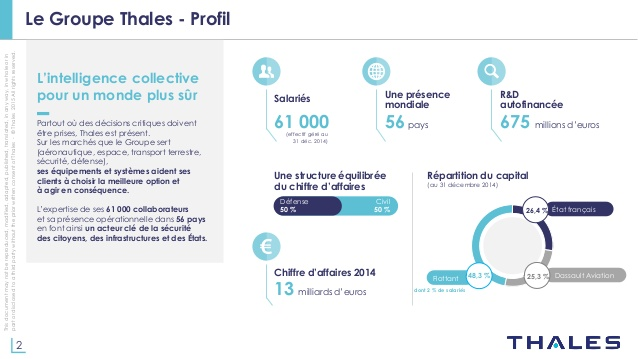
\includegraphics[width=.9\linewidth]{./assets/thales_chiffres}
\caption{THALES en quelques chiffres}
\medskip
\small
\end{figure}
 
\subsection{Description du sujet de stage}
\subsubsection{L'environnement de simulation: SE-STAR}

SE-STAR est un logiciel de simulation dans des environnements modélisés à partir
de lieux réels. Dans l’environnement virtuel interagissent en temps réel des
agents représentant des personnes. Il est conçu en particulier pour les
infrastructures critiques (stations de métro, gares, aéroports).
Il peut gérer en temps réel un grand nombre d’agents (plus de 10 000), permettant de nombreuses interactions avec l’environnement qui peut être facilement modifié par l’utilisateur (ajout d’objets tels que des caméras de surveillance, des distributeurs de boissons, des bancs, etc.). La simulation cherche à représenter de manière réaliste le comportement des usagers de ces infrastructures. 

Dans le contexte de ce stage, nous allons restreindre SE-STAR à la modélisation d'un environnement simple contenant un seul agent. 

\midskip
\begin{figure}[!h]
\centering
\begin{subfigure}{.5\textwidth}
  \centering
  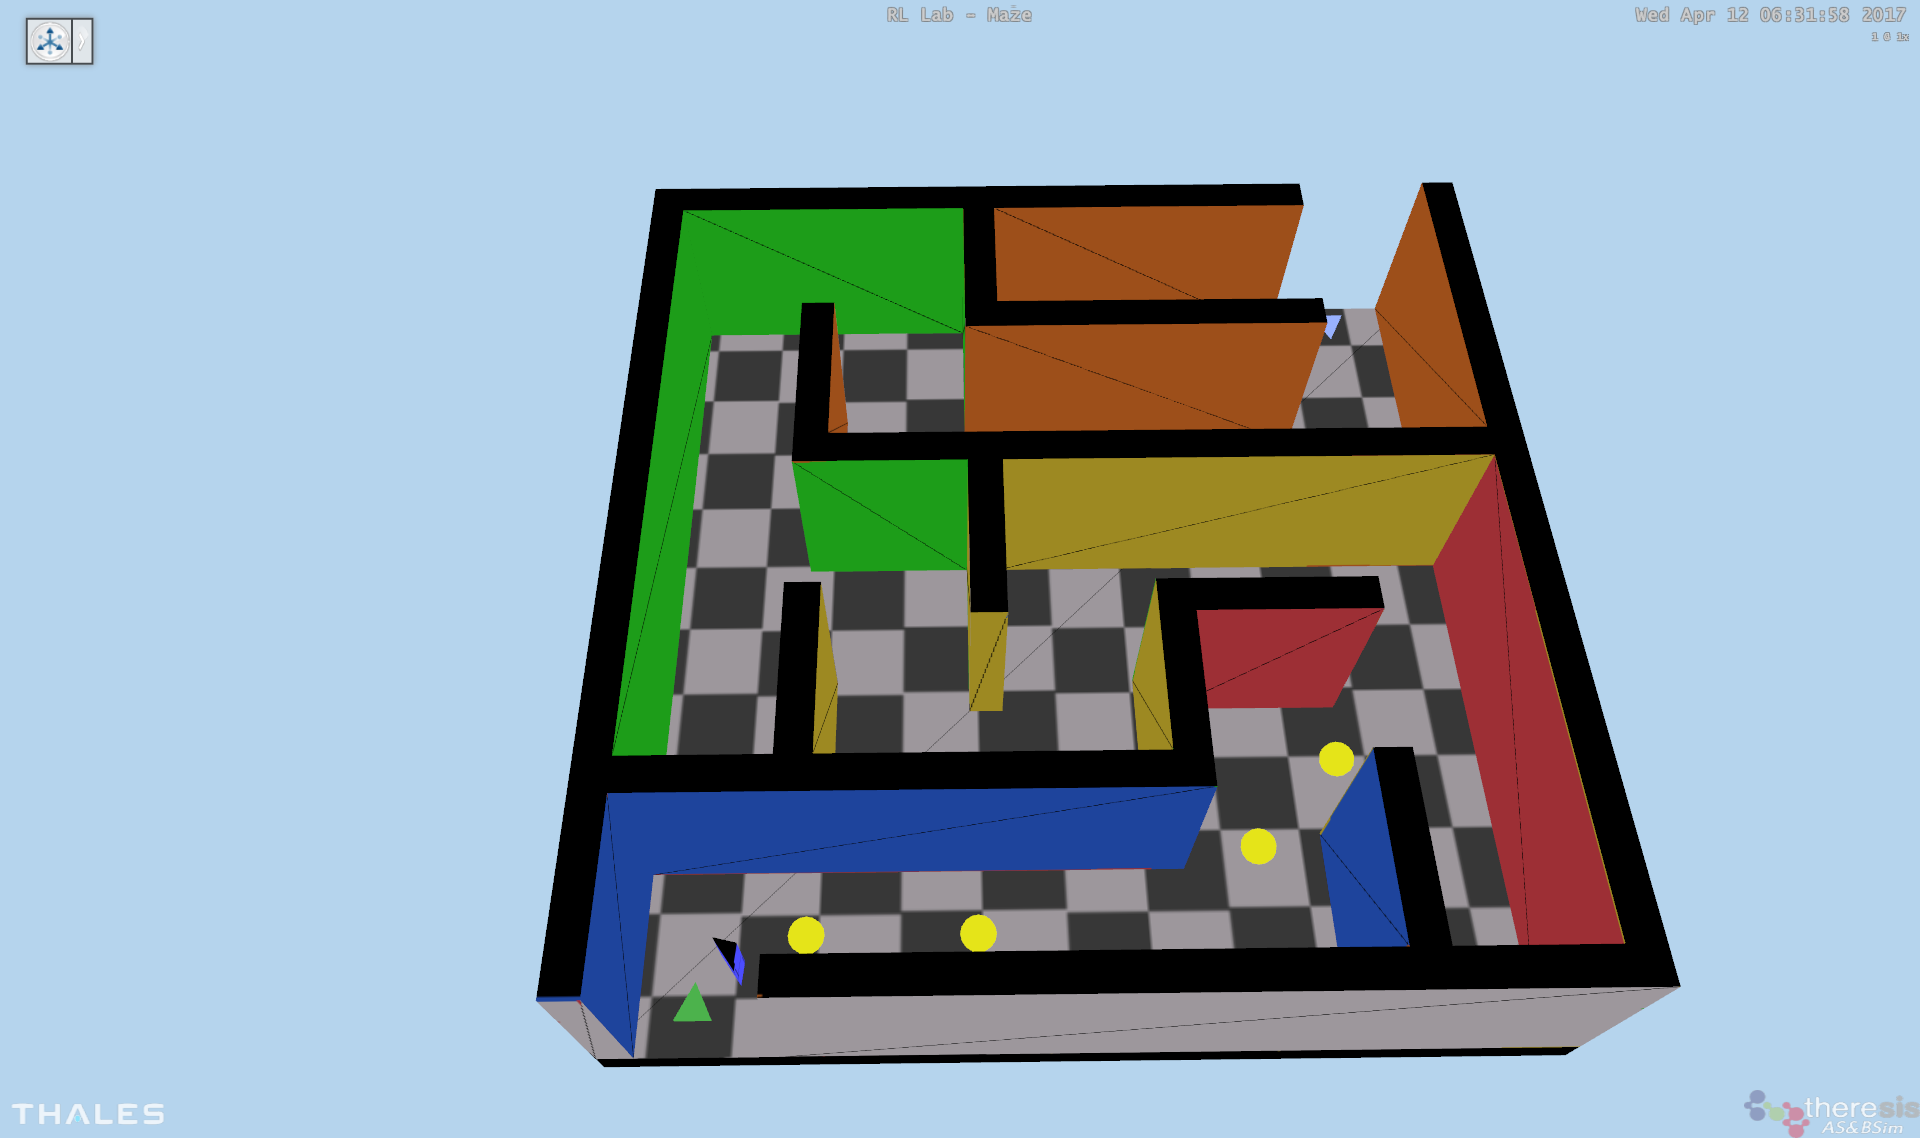
\includegraphics[width=.9\linewidth]{./assets/SESTAR/env_sestar_color.png}
  \caption{Environnement créé pour le contrôle d'un agent}
  \label{fig:sub1}
\end{subfigure}%
\begin{subfigure}{.5\textwidth}
  \centering
  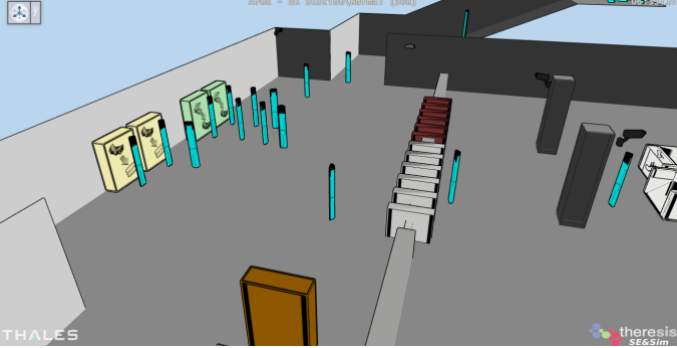
\includegraphics[width=.9\linewidth]{./assets/SESTAR/sestar_metro.png}
  \caption{Simulation d'une station de métro}
  \label{fig:sub2}
\end{subfigure}
\caption{Exemple d'utilisation de SE-STAR}
\label{fig:test}
\end{figure}

\subsubsection{Objectif du stage et contraintes identifiées}


L'objectif de ce stage est de proposer un contrôle d'un agent de l'entrée de l'environnement à la sortie de l'environnement en évitant des zones considérées comme dangereuses. Néanmoins, nous possédons des contraintes sur notre contrôle:     

\begin{enumerate}
    \item \textbf{L'environnement est inconnu de l'agent:}
    \smallskip
    
    La première contrainte de notre objectif est que notre environnement est inconnu. En effet nous souhaitons développer un algorithme de contrôle que soit capable de proposer un asservissement fiable pour tout environnement proposé par SE-STAR. L'impératif de généralisation est une contrainte forte pesant sur le choix technologique pour réaliser ce contrôle. En effet, un asservissement classique repose sur la connaissance de la dynamique du système qui n'est pas disponible dans notre cas et , pire encore, est fluctuante en fonction des environnements.
    
    \item \textbf{Le contrôle doit être robuste aux changements d'environnements:}
    \smallskip
    
    Pour être utile, il faut que notre agent apprenne à se mouvoir d'un point A à un point B. De plus, notre algorithme d'apprentissage ne doit pas se suffire à apprendre par coeur la séquence d'action pour rejoindre la sortie mais doit apprendre à se repérer et voir les points d'intérêts permettant de trouver la sortie quelque soit l'environnement. Nous recherchons une approche analogue à la façon humaine  pour sortir d'un environnement (longer les murs, chercher des indices visuels indiquant la sortie ...).
 
    \item \textbf{Les entrées de la commande sont données par la vision de l'agent:}
    \smallskip
    
    Une des difficultés qui empêche l'utilisation des outils de la théorie du contrôle, vient du format des entrées. Nous devons bâtir un algorithme de contrôle se basant sur des images partielles d'un environnement. Comme un humain lâché dans un labyrinthe, il n'aura pas accès à une image complète du labyrinthe mais uniquement une vue partielle possiblement bruitée. Notre agent devra, à partir d'une information incomplète, réussir à déterminer une séquence d'actions lui permettant de trouver la sortie.
    
  
\end{enumerate}

\subsubsection{Défis et choix technologiques}

Nous cherchons un algorithme de contrôle assez générique pour ne nécessiter en entrée que des images (tableaux de pixels). Un des défi de ce stage est de permettre à  l'agent d'être capable de trouver les repères les plus adaptés pour réussir sa mission quelque soit l'environnement.

Cela implique que nous ne recherchons pas seulement une solution adaptée à un environnement particulier. Nous souhaitons un agent capable de généraliser à un ensemble d'environnements similaires la recherche d'une politique quasi optimale. 

Les nombreuses contraintes et les défis technologiques impliquent une décomposition de l'algorithme choisi en deux grandes étapes:

\begin{enumerate}
    \item L'agent explore l'environnement et apprend simultanément une politique optimale pour arriver à la sortie.
        % coeur -> e dans le o
    \item Nous nous assurons que l'agent est capable de trouver une bonne politique sur des environnements similaires pour vérifier que l'agent n'a pas juste \emph{appris par coeur une solution}.
\end{enumerate}

Se pose naturellement la question du choix de la technologie pour réaliser cet apprentissage.
La contrainte de généralisation nous pousse à utiliser l'apprentissage profond (ou \emph{deep learning}). L'apprentissage profond a prouvé son efficacité dans sa capacité à être pertinent à un grand nombre d'entrées possibles.  
La distinction entre généralisation et apprentissage par coeur des données est particulièrement importante dans ce domaine. Les méthodes qui en sont issues ont prouvé leurs capacité à trouver des solutions à des problèmes nouveaux (jamais utilisés en entrainement).

Il nous faut un domaine s'attaquant à des environnements compliqués, observés de manières partielles, et possiblement changeant au cours du temps. L'apprentissage par renforcement propose une manière d'aborder ce genre d'environnement complexe. 

Ainsi, nous avons proposé une méthode alliant l'apprentissage profond pour gérer les entrées du système avec l'apprentissage par renforcement pour réaliser un agent capable de naviguer dans un environnement pour y découvrir une sortie en ayant comme donnée unique sa vision.

\newpage
\section{Revue de la littérature et état de l'art}

Dans cette partie, nous allons passer en revue les principales explications du fonctionnement de notre contrôleur. 
En particulier, nous expliquerons comment fonctionne l'apprentissage par renforcement, les intérêts de cette technologie et ses limites.  

Nous mettrons en relation l'apprentissage par renforcement avec l'apprentissage statistique (deep learning) comme un moyen de pallier aux limitations de l'apprentissage par renforcement et ses autres bénéfices.

Enfin, nous discuterons des moyens mis en place pour tester nos algorithmes sur des cas moins complexes pour s'assurer du fonctionnement de nos codes.

\subsection{Fonctionnement de l'apprentissage par renforcement et intérêt}

L'apprentissage par renforcement est une sous partie de l'apprentissage automatique. Elle fait référence à un apprentissage qui est à partir d'expériences de façon à optimiser un récompense en cours du temps. A chaque action effectuée par l'agent, l'environnement attribut à celui ci une récompense. L'objectif est de trouver la séquence d'actions qui mène à la plus grande accumulation de récompenses. L'agent va être uniquement guider par son expérience et devrait apprendre de ses erreurs. Imaginons le cas suivant: nous devons apprendre un nouveau tour à notre chien néanmoins, il est impossible de lui exprimer clairement ce que nous souhaitons de lui. Notre seul levier est la quantité de récompenses ou au contraire de punition que va recevoir le chien. Ce problème est connu sous le nom de: \emph{problème d'assignement du crédit}. 

Une dès particularité de l'apprentissage par renforcement réside dans le fait que notre politique d'actions influencent grandement les états rencontrés. Prenons l'exemple d'un agent autonome dans un labyrinthe à la jonction entre deux salles différentes. Si la séquence d'actions fait se retrouver notre agent dans une des salles, il n'aura accès qu'a la vision de cette salle.

\subsubsection{Formalisation de l'approche par renforcement}

Nous allons proposer un formalisme  permettant d'introduire les notions importantes de l'apprentissage par renforcement. Nous commençons par expliquer de façon simple les notions indispensable puis nous nous servirons des processus de décision markoviens pour avoir un cadre solide.

Nous considérerons: 

\begin{itemize}
    \item Un ensemble d'états noté $\bm{\mathbb{S}}$
    
    Cette ensemble d'états regroupe l'ensemble des états possible pouvant être fournis par l'environnement. Dans le cas du jeux d'échecs, cela correspondrait au nombre de positions possibles atteignables ($\sim 10^{43}$ soit un nombre supérieur au nombre d'atomes dans l'univers)
    
    \item Un ensemble d'actions noté $\bm{\mathbb{A}}$
    
    Cette ensemble d'action regroupe les actions possibles par l'agent en fonction de l'état dans lequel il se trouve. Il est possible d'imaginer des états pour lesquelles l'ensemble des actions soit différent. Dans le cas des échecs les actions possibles peuvent différer en fonction de l'état de la partie (exemple: clouage, roi en échec ...).

    \item Un ensemble de récompenses noté $\bm{\mathbb{R}}$
    
    Cette ensemble regroupe les récompenses que peut fournir l'environnement. C'est récompense peuvent être nul, négative ou positive (nous parlerons de récompense quelque soit la valeur de celle ci). Les récompenses dépendent à la fois de l'état mais aussi de l'action effectué par l'agent.
    
    Selon le cas, il peut être à l'expérimentateur de définir une politique de récompense mais dans de nombreux cas l'ensemble de récompense se fixe facilement. Dans le cas de notre labyrinthe l'agent reçoit +1 s'il trouve la sortie 0 sinon. Nous expliquerons plus tard pourquoi cette politique de récompense n'est pas forcement bien adapté.
    
    \item La dynamique de l'environnement $\bm{\mathbb{T}}$
    
    La dynamique de l'environnement représente la probabilité, sachant que j'effectue une action $\bm{a \in \mathbb{A}}$ et que je suis d'en un certain état $\bm{s_t \in \mathbb{S}}$, d'atterrir dans un état  $\bm{s_{t+1} \in \mathbb{S}}$. C'est une connaissance sur le modèle qui dans bien des cas nous fait défaut. En l'occurrence dans notre cas pendant ce stage, la dynamique est une donné non connue. Il est à noter que ce qui est précédemment énoncé n'est vrai que sous l'hypothèse de Markov qui nous assure que notre dynamique est conditionnellement indépendante de  des états et actions précédents. Cette hypothèse est fausse en pratique et nous discuterons des stratégies utilisées pour pallier à ce problème. 
    
    \item La politique d'action $\bm{\Pi}$
    
    La politique d'action peut être défini comme la probabilité, sachant que je suis dans un certain état $\bm{s_t \in \mathbb{S}}$, d'effectuer une action $\bm{a \in \mathbb{A(s_t)}}$.
    Dans un soucis de généralité, nous considérons une politique stochastique néanmoins la politique peut être déterministe. En apprentissage par renforcement nous cherchons à optimiser notre politique d'action dans le but de maximiser la quantité de récompense.
        

\end{itemize}

Ainsi un problème d'apprentissage par renforcement profond classique suit le schéma suivant. A chaque pas de temps t, l'agent va percevoir un état $\bm{s_t \in \mathbb{S}}$. L'agent va choisir l'action à effectuer $\bm{a \in A(s_t)}$ et va recevoir une récompense $\bm{r_{t+1}}$. Notre objectif va donc être de maximiser la somme pondérée des récompenses obtenues par notre séquence d'actions. 


On définira notre problème sous la forme d'un processus décisionnel de Markov, soit un 5-tuple $\bm{\big(\mathbb{S}, \mathbb{A}, \mathbb{T}, \mathbb{R}, \gamma \big)}$.

Notre objectif est de trouver la politique $\bm{\Pi}$ tel que la somme pondérée des récompenses (notée $\bm{G_t}$) soit maximale avec:

\begin{align}
G_t = \discountedReward \quad \text{sachant} \quad a_t = \Pi(s_t)
\end{align}

Pour déterminer la politique optimal, il est utile de définir la fonction de valeur d'états $\bm{V(s_t)}$ qui représente le gain moyen à partir d'un certain état en suivant une  politique $\bm{\Pi}$ et la fonction de valeur d'états actions $\bm{Q(s_t, a_t)}$ qui représente le gain moyen à partir d'un certain état et en effectuant une certaine action puis suivant une  politique $\bm{\Pi}$.
\begin{gather}
\quad V(s_t) = \valueFunction \\[.1cm]
\quad  Q(s_t,a_t) = \QFunction
\end{gather}


Une propriété fondamentale des fonctions d'état et d'état-action est qu'ils respectent une relation de récursivité bien connu: l'équation de Bellman (pour $V$ et $Q$):

\begin{gather}
V_\pi(s_t) = \underset{a}{\bsum}\: \policyc{blue} \:\underset{s', r}{\bsum}\:\dynamicsc{red}\: \bigg[\: r + \gamma V_\pi(s') \:\bigg] \\
Q_\pi(s_t, a_t) = \underset{s', r}{\bsum}\:\dynamicsc{red}\: \bigg[\: r + \gamma V_\pi(s') \:\bigg] 
\end{gather}

\bigskip

les relations précédentes sont particulièrement intéressantes car elles nous permettent d'exprimer la valeur d'un état à partir de la valeur des états successifs à celui ci. Nous pouvons représenter sous forme d'un graphique la relation précédentes:

:: IMAGE

Ces deux relations sont à l'origine de nombreuses méthodes en apprentissage par renforcement. Notamment, elles seront à l'origine des méthodes appliquées pendant ce stage dans le contrôle d'un agent dans la simulation de Thales SE-STAR.

Pourtant, nous n'avons toujours pas explicité la forme de la politique optimale. Nous allons nous aider des fonction d'état, et d'état-action qui fournisse un indicateur sur la pertinence de la politique choisie. Ainsi, on pourra dire qu'une politique $\pi$ est meilleurs qu'une politique $\mu$ si $V_\pi(s) > V_\mu(s), \forall s $. Il parait donc intéressant de rechercher la politique maximisant la fonction d'état $ V_* = \underset{\pi}{\max} \:V_\pi(s) $. On peut faire la même chose avec la fonction d'état-action: $ Q_* = \underset{\pi}{\max} \:Q_\pi(s, a) $.

Nous pouvons explicité $Q^*$ et $V^*$ correspondant aux équations optimales de Bellman respectives:

\begin{gather}
V^*(s) = \underset{a}{\max} \: \underset{s', r}{\bsum} \: p(s',r \vert s, a) \bigg[\: r + \gamma V_\pi(s') \:\bigg]
\\
Q^*(s, a) = \underset{s', r}{\bsum} \: p(s',r \vert s, a) \bigg[\: r + \gamma \: \underset{a'}{\max} \: Q_\pi(s', a') \:\bigg]
\end{gather}
\bigskip

:: IMAGE

A partir des fonctions état et état-action, il est relativement aisé de déterminer la politique optimale. Une fois qu'on a déterminé $V^*$ nous pouvons déterminer l'action optimal en faisant une recherche à un pas dans le temps. Ce qui est remarquable est qu'en apprentissage par renforcement, il y a un compromis fondamental entre un objectif à court et long terme pourtant nous venons d'affirmer qu'en exploitant $V^*$ et en faisant notre recherche à un pas nous avons pris compte des effets à long termes. Avec la fonction d'état-action c'est encore plus simple car il n'y a plus besoin de recherche auxiliaire car la fonction d'état-action encode déjà cette recherche, il suffit donc d'exploiter la fonction d'état-action optimale à chaque action pour obtenir la politique optimal: $\pi^*(s) = \underset{a}{\max}\:Q^*(s,a)$ 

Malheureusement, il est, dans la plupart des cas, impossible de déterminer les fonctions d'états ou d'états-actions optimales car cela reviendrait à une recherche exhaustive de toutes les possibilités avec la connaissance de leurs probabilités d'apparaître et la connaissance du gain espéré associés. Néanmoins, les fonctions d'état et d'état-action sont utiles à l'apprentissage et au contrôle de notre agent. Dans la partie suivante nous allons expliquer comment approximer ces fonctions pour pouvoir commencer à établir des algorithmes de contrôle efficace.
\bigskip
\begin{tcolorbox}[colback=gray!5!white,colframe=red!65!white,title=L'apprentissage par renforcement en résumé, coltitle=black, fonttitle=\bfseries]

L'apprentissage par renforcement propose de contrôler un agent grâce à des stimulis (récompenses) données par l'environnement ou l'expérimentateur. \\

L'objectif est de déterminer une politique (soit un fonction $\mathbb{S} \: \rightarrow \: \mathbb{A}$) qui maximise le gain cumulé pondéré (pondération utile pour favoriser l'importance des récompenses à court termes tout en prenant en compte les récompenses à long termes).\\ 


Pour déterminer la politique optimale, nous nous aidons de deux fonctions (les fonctions d'états et d'états-actions) qui sont une mesure de la quantité de récompenses pouvant être espéré à un certain état (ou à un état en effectuant une certaine action) en suivant une politique. 

On peut dès lors en trouvant une fonction d'états (ou d'états-action) optimales dérivé une politique optimale. \\

Sauf cas jouet, les fonctions d'états (états-actions) sont inconnus, notre objectif va être de trouver une façon de les approximer pour permettre l'établissement d'algorithme de contrôle par apprentissage par renforcement.\\


Enfin, nous montrerons que nous ne sommes pas obliger de passer par ce proxy pour déterminer la politique optimale tout en insistant que la connaissance des fonctions d'états est un atout quelque soit l'approche utilisé.
\end{tcolorbox}
\subsubsection{Introduction des principales approches en apprentissage par renforcement}

Après avoir introduit les principaux concepts de l'apprentissage par renforcement, il convient d'en extraire des algorithmes permettant de trouver notre politique optimale. Un difficulté majeur est que nous n'avons ni connaissance des fonctions d'états (et d'états-actions) ni connaissance de la dynamique du modèle (noté $\textcal{T}$).

La question est donc de savoir s'il est possible d'approximer ces fonctions, ou alors de s'en passer.

Avant de répondre à ces questions, il est important de faire la différence entre deux types d'approches en apprentissage par renforcement: 

\begin{enumerate}
    \item \textbf{Model Free} (Apprentissage sans modèle): \\
    Dans ce type d'approche, nous n'utilisons pas un modèle de l'environnement pour déterminer la politique optimale, uniquement une recherche basée sur notre expérience. Intuitivement, on pourrait penser cette approche inférieur à l'approche \emph{Model Based} pourtant on verra que l'approche \emph{Model Free} est plus simple à mettre en place et est plus performante dans la plupart des cas que nous avons rencontré. Cela s'explique par la difficulté d'apprentissage de la dynamique de l'environnement (qui dans bien est cas n'est pas stationnaire).
    
    \item \textbf{Model Based} (Apprentissage avec modèle): \\
    Dans ce type d'approche, nous allons utiliser la connaissance du modèle (ou l'approximation interne du modèle par l'agent) pour déterminer la politique optimale. L'apprentissage avec modèle apparaît comme plus puissant mais est encore un problème non résolus (tout comme en Model Free mais des algorithmes ont déjà montré leur capacité à résoudre des environnements difficiles). La difficulté étant que bien souvent l'entrée n'est pas très informative sur la dynamique de l'environnement. Ainsi, une image 2D représentant un monde 3D est une entrée dont il est difficile de tiré un modèle. 
\end{enumerate}

Dans cette partie, nous allons nous concentrer sur l'établissement d'algorithme \emph{Model Free}. 


Précédemment, nous avons établi que nous n'avions aucune connaissances des fonctions d'états, ni de la dynamique de l'environnement. Notre objectif est trouvé une approximation des fonctions optimales d'états qui nous permettrait d'établir une politique optimale. Pour ce faire nous devons trouver un moyen d'approximer la fonction d'état et de trouver un moyen d'établir à quelle point notre approximation est loin de la fonction optimale.

Nous expliquerons plus tard le mécanisme d'approximation de fonctions utilisé (réseau de neurone), pour cette partie, nous considérerons juste la fonction $\omega, s \rightarrow \overset{\sim}{V_\omega}(s)$ qui associe une matrice $\omega$ et un état à une approximation de la fonction d'état. 

Nous pouvons ainsi formaliser, en un problème d'optimisation, notre objectif:

$$ \omega^* = \underset{\omega}{\min} \norm{{V^\pi - \overset{\sim}{V}_\omega}}_2$$

On peut donc en utilisant une méthode d'optimisation tel que la descente de gradient stochastique déterminer un minimum locale:

\begin{equation}
\begin{aligned}
\omega_{t+1} = \omega_t - \tfrac{1}{2} \: \alpha \nabla_\omega \norm{{V^\pi - \overset{\sim}{V}_\omega}}_2 \\[0.75ex]
\omega_{t+1} = \omega_t + \tfrac{1}{2} \: \alpha (V^\pi - \overset{\sim}{V}_\omega)\nabla_\omega \overset{\sim}{V}_\omega

\end{aligned}
\end{equation}

Cela nous pose un problème de taille, nous n'avons pas connaissance de la fonction d'état or notre précédante équation repose sur la connaissance de celle ci et ils ne seraient pas pertinant de chercher une approximation d'une fonction déjà connue. Il existe plusieurs méthodes pour l'approximer, nous allons en donner deux. Une méthode basé sur la méthode de Monte Carlo, et l'autre basé sur du \emph{bootstrapping} (le bootstrapping étant basé sur des processus itératifs convergeant vers la valeur qui est souhaitée)

\bigskip 

\begin{center}

\setlength{\tabcolsep}{10pt}
\renewcommand{\arraystretch}{1.5}
 
\begin{tabular}{ |c|c|  }
\hline
\multicolumn{2}{|c|}{Approximations possibles de la fonction d'état} \\
\hline
Monte-Carlo &  $\overset{\sim}{v}(s_t) = \mathbb{E}_\pi \big[G_t \vert S_t = s\big] \sim \frac{1}{N}\:\underset{k=0}{\sum}^N\: \gamma r_{t+k}$
\\[1.5ex]
\hline
Bootstrapping & $v_{k+1} =  \underset{a}{\sum}\: \pi(a, s)\: \underset{s', r}{\sum} \:p(s', r \:\vert\: s, a) \: \big[ r + \gamma\: v_k(s')\:\big]$  \\

\hline
\end{tabular}
\end{center}

\bigskip 

Nous commencerons par envisager l'approche par bootstrapping. La première remarque est que le bootstrapping requiert la connaissance du modèle de l'environnement ce qui est particulièrement handicapant dans notre cas. Néanmoins, nous avons des garantis sur la convergence de notre approximation vers la fonction d'état. Ainsi, si nous sommes en capacité de connaître le modèle, il nous suffit d'itérer pour connaître la véritable fonction d'état. Pourtant, le véritable problème que nous avons avec cette méthode est un problème qui apparaîtra souvent et qui est dénommé \emph{la malédiction de la dimensionalité}. Plus la dimensionnalité de l'état est grande plus le coût de cette approche augmente (de façon exponentielle). Dans notre cas d'usage, l'état sera un tableau de pixel ce qui rend impossible l'utilisation de ce genre d'algorithmes.

Si l'approche précédente reste inapplicable, la philosophie du bootstrapping n'a pas a être jeté. Il n'est pas pertinent de rechercher à tendre vers la fonction d'état en itérant selon la formule de bellman, cependant il sera intéressant de chercher à itérer d'une autre façon de façon à s'approcher de la véritable fonction d'état. Toute la question est de trouver une formule qui permet d'itérer (à faible coût) et qui garantie de tendre vers une approximation de la fonction d'état pertinente.


Passons maintenant à la méthode via \emph{Monte Carlo}. Cette méthode s'intègre parfaitement dans l'esprit de l'apprentissage par renforcement. En effet, un agent va jouer un épisode et récupérer un ensemble d'action, état, et récompense. A partir de cet ensemble, nous sommes en capacité d'approximer la fonction d'état tel que l'approximation de la fonction d'état pour un état s correspond aux récompenses obtenues dès la première visite de l'état s (\emph{First visite Monte Carlo}). Dans le cas où on va jouer plusieurs épisode, on pourra affiner notre approximation en approximant notre fonction d'état pour un état s comme étant la moyenne des récompenses obtenues dès la première visite de l'état s sur l'ensemble des épisodes joués. 
Les méthodes d'approximations de la fonction d'états possède des quelques avantages par rapport au bootstrapping:

\begin{itemize}
\item Insensible à la dimension de l'état ce qui est intéressant dans notre cas.
\item On peut générer des épisodes en commençant par les états nous intéressant pour estimer leur fonction d'état ce qui n'est pas possible.
\end{itemize}

Néanmoins, l'approche par Monte Carlo possède aussi des désavantages tel que le fait d'être obliger de jouer un épisode entier pour pouvoir estimer la fonction d'état. Cela pourra être problématique dans le cas où l'épisode est  long . De plus, il parait pertinent de pouvoir itérer à partir d'estimations antérieures ce qui n'est pas le cas avec les méthodes de Monte Carlo. 

\subsubsection{TD Learning: la base des algorithmes pour le contrôleur}
\todo[inline]{explain temporal difference --> td}
 En se basant sur l'approximation décrite précédemment en utilisant l'approche de Monte-Carlo. Pour un environnement non stationnaire (qui change en fonction du temps), on peut trouver une formule approximant la fonction d'état:
 
 \begin{equation}
\overset{\sim}{V}_{\pi}(S_t) \leftarrow \overset{\sim}{V}_{\pi}(S_t) + \alpha \bigg(\textcolor{blue}{G_t} - \overset{\sim}{V}_{\pi}(S_t)\bigg)
\end{equation}
 
Le problème de la formule ci dessus est que pour mettre à jour notre croyance sur la fonction d'état, nous sommes obligé d'attendre la fin d'un épisode.

Nous allons voir dans cette partie qu'il est possible de combiner les approches de Monte-Carlo et Bootstrapping pour garder les avantages dès deux méthodes tout en gommant leurs défauts. Pour cela, rapellons la formule de la fonction d'état: 

\begin{align*}
V_{\pi} = \valueFunction \\
= \mathbb{E}_\pi \big[\textcolor{blue}{G_t} \vert S_t = s\big] \\
= \mathbb{E}_\pi \big[\textcolor{red}{r_{t+1} + \gamma V_{\pi}(S_{t+1})} \vert S_t = s\big]
\end{align*}
 
 On peut en déduire une nouvelle formule pour pour estimer la fonction d'état:
 
\begin{equation}
\overset{\sim}{V}_{\pi}(S_t) \leftarrow \overset{\sim}{V}_{\pi}(S_t) + \alpha \bigg(\textcolor{red}{r_{t+1} + \gamma V_{\pi}(S_{t+1})} - \overset{\sim}{V}_{\pi}(S_t)\bigg)
\end{equation}

Nous obtenons ainsi une formule se basant sur du bootstrapping car nous nous servons de la fonction d'état à $S_{t+1}$ et nous n'avons toujours pas besoin de la connaissance du modèle (Monte-Carlo).

La formule précédemment constitue la base sur laquelle on va s'appuyer pour créer notre contrôleur néanmoins si la fonction d'état est importante, il est plus intéressant d'approximer la fonction d'état action dans le contexte d'un contrôle.

Pour le contrôle, c'est donc la formule ci dessous, qui se nomme SARSA (pour \emph{state action reward state action} \footnote{voir la formule ci dessous pour comprendre pourquoi}, qui sera utilisé:

\begin{equation}
\overset{\sim}{Q}_{\pi}(S_t, A_t) \leftarrow \overset{\sim}{Q}_{\pi}(S_t, A_t) + \alpha \bigg(r_{t+1} + \gamma \overset{\sim}{Q}_{\pi}(S_{t+1}, A_{t+1}) - \overset{\sim}{Q}_{\pi}(S_t, A_t)\bigg)
\end{equation}

Il existe dans la littérature une pléthore de variation de SARSA en particulier, une des variations qui va nous intéresser est celle qui s'appelle Q-Learning \cite{Watkins92q-learning}: 

\begin{equation}
\overset{\sim}{Q}_{\pi}(S_t, A_t) \leftarrow \overset{\sim}{Q}_{\pi}(S_t, A_t) + \alpha \bigg(r_{t+1} + \gamma \underset{a'}{\max}\overset{\sim}{Q}_{\pi}(S_{t+1}, a') - \overset{\sim}{Q}_{\pi}(S_t, A_t)\bigg)
\end{equation}

Malgré leur relative proximité, nous privilégierons le Q-Learning pour dès raison que nous expliquerons plus tard. 

Nous allons finir cette partie sur le TD Learning par expliquer la relation entre l'approximation de la fonction d'état par optimisation d'une fonction de perte et le Q learning. Cette introduction est importante car c'est l'algorithme le plus simple qui a été utilisé durant ce stage sur différent environnements. Nous allons expliquer comment fonctionne le Deep Q Learning \cite{2013arXiv1312.5602M} \cite{mnih-dqn-2015} (soit le premier algorithme d'apprentissage par renforcement profond). 

Néanmoins, nous n'expliquerons pas totalement cette algorithme car il requiert quelques connaissances en deep learning pour la compréhension du mécanisme d'approximation de la fonction. Pourtant, il est important de le mentionner maintenant car il découle du TD Learning et en particulier de l'algorithme du Q-Learning et qu'il est fondamental pour la compréhension des autres algorithmes utilisés durant ce stage.

\subsubsection{Du TD Learning au Deep Q Learning}

Un problème en apprentissage par renforcement est la représentation de la fonction d'état (d'état action). Naivement, on pourrait imaginer un dictionnaire qui à chaque état garderait en mémoire la fonction d'état action pour chacune des actions néanmoiNs dans le cas d'états représentés par des pixels, il faudrait une capacité astronomique de mémoire pour cela. 

Nous préférons donc utiliser des fonctions paramétrisées par un ensemble de poids (noté $\theta$) tel que $f_\theta = \overset{\sim}{Q} \sim Q$. 

Précédemment, nous avions introduit une méthode par optimisation d'une fonction de perte pour permettre de trouver l'ensemble $\theta$ tel que $f_\theta = \overset{\sim}{Q} \sim Q$. 

Imaginons maintenant que notre agent joue dans l'environnement et récolte des transitions (un ensemble composé de l'état courant, de l'état précédent, de l'action jouée et de la récompense obtenu que l'on notera $e_i$ pour la ième transition). L'agent stockera ces transitions dans une mémoire que l'on notera $\mathcal{D}$. Soit $\mathcal{D} = \big(e_0, ..., e_N\big)$ 

La fonction de perte utilisée est: 
\begin{align}
L_i(\theta_i) = \mathbb{E_{\text{s}, \text{a} \sim \rho(.)}}\bigg[ \big( y_i - f_\theta(s, a; \theta)\big)^2 \bigg]\\
y_i = \mathbb{E}_{\text{s'} \sim \Epsilon}\big[r + \underset{a'}{\max}f_{\theta_{i-1}}(s', a') \big] 
\end{align}

Avec $\rho(s, a)$ la distribution sur la séquence d'états et d'actions.
\subsubsection{Platforme utilisables pour garantir le fonctionnement de nos algorithmes}

Malgré que nos algorithmes aient pour but d'être déployer sur l'environnement interne de Thales SE-STAR, il nous a fallut trouvé des environnement suffisamment complexe pour tester la robustesse de nos agent mais aussi suffisamment simple pour ne pas devoir un temps infiniment long pour avoir notre réponse. De plus, la connection de nos algorithmes avec SE-STAR est un enjeu essentielle et a apporté son lot de difficulté. Il n'était donc pas raisonnable d'attendre ni de tester nos agents sur cette plateforme.

Il existe de nombreuses plateformes dédiées à l'apprentissage par renforcement. Nous avons choisis de nous concentrer sur des environnements proches de SE-STAR. Ainsi, de nombreuses études en RL utilise des jeux Atari en 2D et 3D. Nous allons donc nous basé en partie sur ce type d'environnement.

Vous pouvez voir page suivante plusieurs types d'environnements sur des plateformes différentes:

\begin{enumerate}
    \item \textbf{Gym\cite{1606.01540} - OpenAI}\\
    Gym est une plateforme qui met à disposition des jeux Atari et des simulations typiques en contrôle (Cartpole, MountainCar ...). La plateforme fournit une API permettant de réutiliser nos codes sur l'ensemble des simulations qui sont fournis par Gym.
    
    L'API de Gym étant simple, nous avons décider de nous basé sur cette API pour la construction d'un wrapper autour de la simulation interne de Thales SE-STAR.
    
    \item \textbf{Universe - OpenAI}\\
    Universe est une autre plateforme mettant à disposition une multitude de jeux très différents les uns des autres (2D, 3D, textes ...). Certains sont récents et demande une certaines réflexions (Portal, age of empire, ...). l'organisation de Universe est plus complexe que celle de gym et impose la prise en compte de plus d'éléments (réseau, possible lag, infrastructure ...). 
    
    Universe propose donc des environnements plus difficiles à tout point de vue que Gym néanmois cette plateforme n'est pas encore utilisé par les chercheurs et on peut douter de la maintenance du projet Universe (OpenAI semble mettre en avant Gym)
    
    \item \textbf{DeepmindLab\cite{DBLP:journals/corr/BeattieLTWWKLGV16} - Deepmind / Google }\\
    Le deepmindlab est une seul simulation de labyrinthe 3D très proche de notre application. Le problème est la difficulté d'utilisation de cette plateforme. Ainsi, nous n'avons pas utilisé cette ressource néanmoins elle est pertinant et est une cible pour tester nos algorithmes.
    
    \item \textbf{Doom - Vizdoom\cite{DBLP:journals/corr/KempkaWRTJ16}  }\\
    Doom est un jeu PC de tir à la première personne. Cet environnement est devenu un classique dans la communauté RL pour tester les algorithmes. A tel point que l'université de Poznan à créer une compétition d'IA basée sur Doom. L'intérêt de ce environnement contrairement au précédant et qu'il est plus complet avec un ensemble d'actions possibles conséquent. De plus, l'environnement de Doom met en lumière des difficulté pour les IA en matière d'exploration de l'environnement et est donc un terrain de jeu pour résoudre ou proposer des algorithmes résolvant ce type de problème.
    

\end{enumerate}

\bigskip
\begin{figure}
\centering
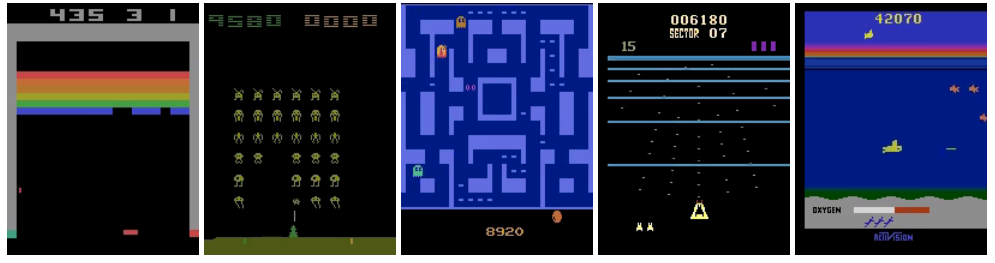
\includegraphics[width=.9\linewidth]{./assets/GYM/gym2}
\caption{Exemple d'environnements GYM (Open AI)}

\bigskip

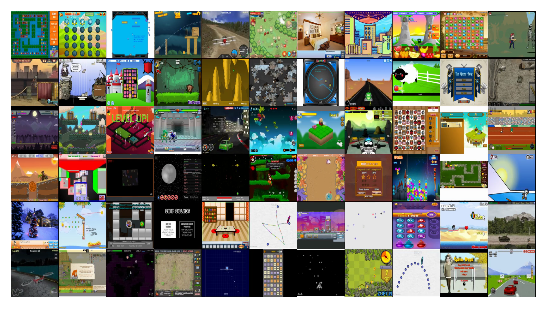
\includegraphics[width=.9\linewidth]{./assets/GYM/gym}
\caption{Exemple d'environnements Universe (Open AI)}

\bigskip

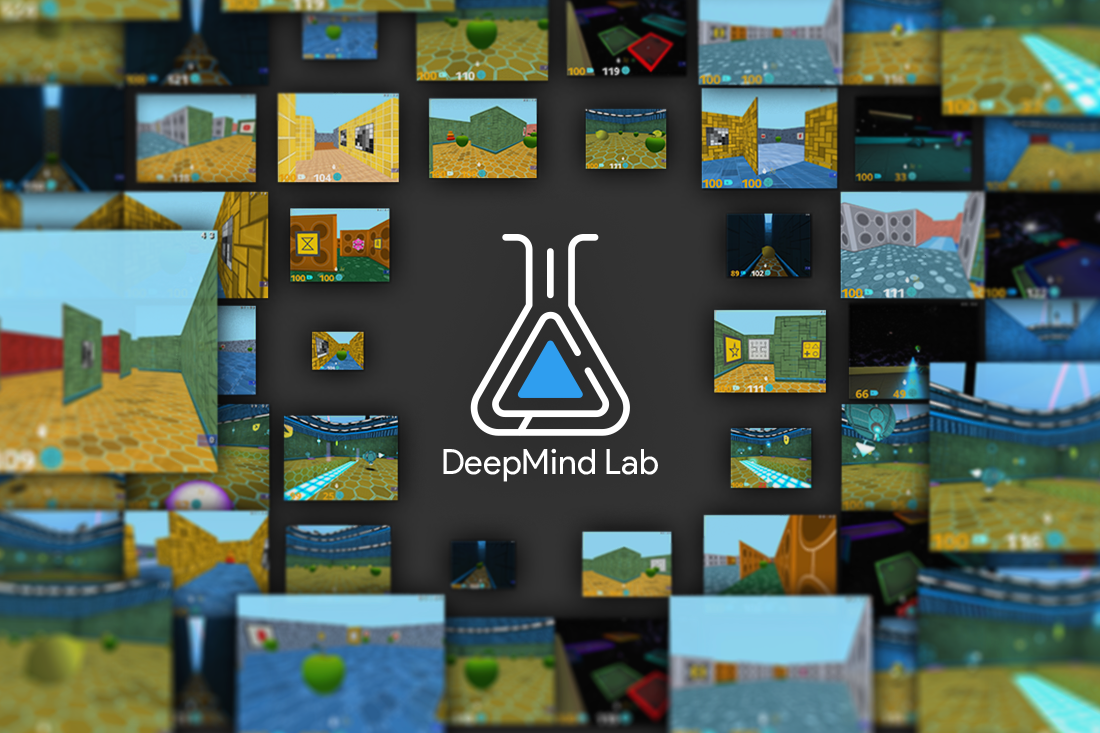
\includegraphics[width=.6\linewidth]{./assets/GYM/deepmindlab}
\caption{Exemple d'environnements DeepmindLab (Deepmind (Google)) }
\medskip
\small
\end{figure}



\subsection{Utilisation et intérêt de l'apprentissage statistique - Deep Learning }

Dans cette partie, nous allons intéresser aux différentes motivations qui nous ont poussé à utilisé l'apprentissage statistique (ou Deep Learning) dans notre contrôleur. Dans notre introduction, nous avons énoncé quelques points qui nous ont influencé pour choisir cette technologique. Nous préciserons en quoi le Deep Learning est pertinent dans notre contexte et introduirons ses principaux concepts et comment l'incorporer avec l'apprentissage par renforcement.

\subsubsection{Motivation et objectif de l'apprentissage statistique}

Nous avons en introduction énoncé les principales contraintes qui reposées sur notre asservissement. De façon synthétique, nous avions trouvé:
\begin{itemize}
\item Environnement partiellement observable (possiblement bruité)
\item Agent doit être capable à partir d'un apprentissage sur une environnement d'être capable de réussir sur un environnement assez proche (généralisation)
\item Les entrées seront basées sur la vision de l'agent
\end{itemize}

Nous verrons que ces problématiques sont abordés par l'apprentissage statistique. La force du deep learning réside dans ça capacité à extraire de l'information à partir d'entrées bruitées à hautes dimensions. Néanmoins, le deep learning possède son lot de restriction parmi lesquels: 

\begin{itemize}
\item Cela nécessite de très nombreux exemples pour réussir son apprentissage.\\nous verrons qu'en RL il faudra parfois plus de $80*10^6$ d'images pour finir un apprentissage)
\item L'apprentissage est difficile et parfois non stable\\nous approfondirons ce point plus tard, mais il est à noter que selon l'architecture choisit et nos fonctions de pertes, la stabilité du réseau n'est pas garanti. De façon plus claire, il y a énormément de facteurs jouant sur la stabilité du réseau et il peut être difficile de régler ces facteurs pour obtenir de bon résultat. 
\item Le réseau peut sur apprendre (apprentissage par coeur des résultats) impliquant l'impossibilité de généraliser.
\end{itemize}

Malgré les difficultés énoncées, le deep learning rend possible notre contrôle basé sur la vision en temps réel d'un agent. 

Définissons le contexte dans lequel le deep learning s'inscrit. A chaque pas de temps, l'agent va recevoir l'image partielle de l'environnement (soit un tableau de pixels). Nous souhaitons en sortie avoir la probabilité d'actions selon l'état (soit la politique pour l'état rencontré).

\begin{center}

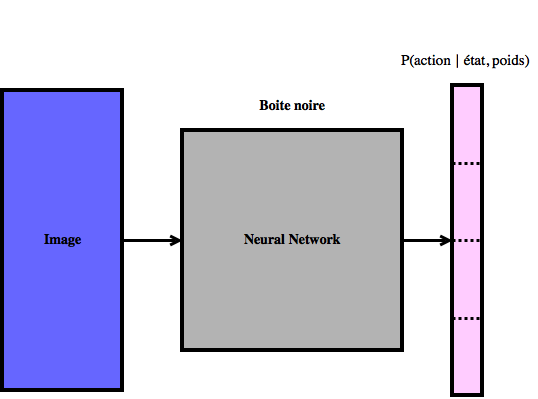
\includegraphics[width=.4\linewidth]{./assets/DeepLearning/dl}
\captionof{figure}{Représentation haut niveau de l'architecture classique en deep learning}
\end{center}

Bien évidemment, le deep learning peut être utiliser pour bien d'autre chose mais nous nous restreindrons à son utilisation dans le cadre de l'apprentissage par renforcement. Néanmoins la figure ci dessus reste d'actualité dans la cadre d'un apprentissage supervisé (exemple en classification: déterminer le nombre représenté par une image correspondrait à avoir en sortie du réseau $P(\text{nombre} \:\vert\: \text{état}, \text{poids)}$. 

Un problème est maintenant de définir comment va être générer  $P(\text{action } \:\vert\: \text{ état}, \text{poids)}$ et c'est là qu'apparait la véritable force du deep learning. On peut façonner automatiquement les poids du réseau de neurone dans le but d'optimiser une fonction de perte (ou de gain).

\begin{center}
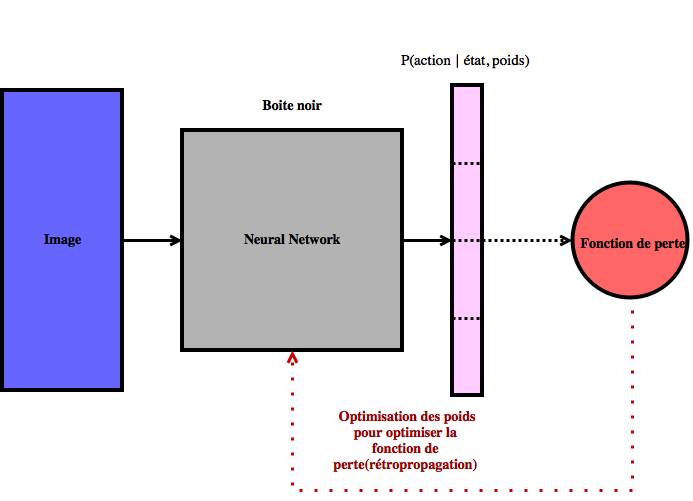
\includegraphics[width=.55\linewidth]{./assets/DeepLearning/dl2}
\captionof{figure}{Représentation haut niveau de l'architecture classique en deep learning avec optimisation de la fonction de perte}
\end{center}
\end{center}

Dans la partie suivante, nous expliquerons les mécanismes responsables de l'optimisation du de la fonction de perte pour véritable  définir ce que veut dire un apprentissage dans le contexte du deep learning. Nous commencerons par introduire ce qu'est un réseau de neurone dans sa forme la plus simple et nous expliquerons succinctement les évolutions utilisées (qui sont le réseau de neurone à convolution et les réseaux récurrents).
\todo[inline]{Revoir - moins de itemize
expliquer l'utilisation des fonctions de coût avant}

\subsubsection{Architecture en apprentissage statistique et réseau de neurone linéaire}

Nous allons commencer par expliquer la structure sur laquelle se base les réseaux de neurones (du moins historiquement) avec \emph{le modèle du perceptron}. 

On définira un ensemble de poids $w$ sous la forme d'un vecteur de poid $W$, l'entrée sera un vecteur $X$ de même dimension que les poids. On appelle $f$ la fonction d'activation qui est une fonction de $\mathbb{R}$ dans $\mathbb{R}$. La fonction d'activation est un hyperparamètre, c'est à dire que c'est à l'expérimentateur de la définir, on retrouve néanmoins quelques fonctions d'activations très utilisées, nous reviendrons sur l'intérêt des fonctions d'activations un peu plus tard. Dans le cas du perceptron, nous utiliserons la fonction d'activation $f(x) = \left \{
  \begin{tabular}{cc}
  +1 \text{si} W^TX > \theta &  \\
  -1 &  
  \end{tabular}
$

\begin{center}
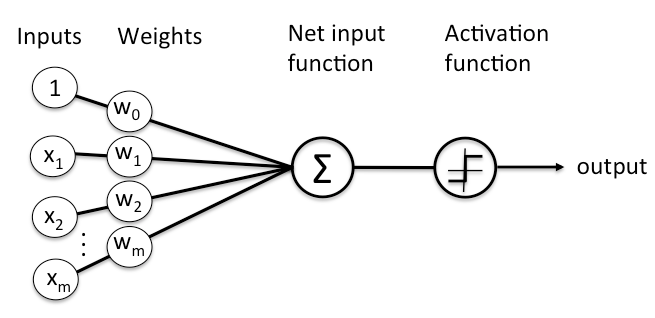
\includegraphics[width=.55\linewidth]{./assets/DeepLearning/perceptron_node}
\captionof{figure}{Représentation haut niveau de l'architecture classique en deep learning avec optimisation de la fonction de perte \cite{blogPerceptron}}
\end{center}


Pour se conformer à la figure 7, il nous reste à définir quelle est la fonction de coût et comment se passe le processus d'optimisation de la fonction de coût. Pour cela, nous avons encore besoin de quelques définitions. Plaçons dans un problème à deux classes (chien et chat par exemple) on définira la classe d'une entrée comme état la classe à laquelle l'entrée appartient ainsi on donnera $c(x) = \left \{
  \begin{tabular}{cc}
  1  \text{si} x \in \text{Chien}  &  \\
  -1 \text{si} x \in \text{Chat}&  
  \end{tabular}
$, cela nous permet donc de définir la façon dont on va optimiser les poids: 
$$ W_{t+1} = W_t - \alpha \big( c(x) - f(x) \big) x $$

\subsubsection{Réseau de neurones dense}
Dans cette partie, nous allons expliquer l'architecture de base utilisée dans le contrôle de l'agent.

Notre objectif est d'approximer une certaines fonction $y = f(x)$. Nous avons accès à un ensemble de entrées et sorties associées que l'on notera $\mathcal{D} = \bigg\{(x_1, y_1), ..., (x_N, y_N)\bigg\}$. Nous souhaitons déterminer la fonction $\overset{\sim}{f}_w$ tel que $\overset{\sim}{f}_w \sim f$, la fonction $\overset{\sim}{f}_w$ est défini comme $\overset{\sim}{f}_w(x) = Wx + b $. Nous pouvons alors de façon équivalent défnir notre objectif comme un problème d'optimisation où l'objectif est de minimiser l'erreur quadratique moyenne $E = \overset{N}{\underset{p=1}{\sum}}\:\big( \overset{\sim}{f}(x) - f(x) \big)^2$. Nous pouvons dès lors changer les poids dans le but de minimiser cette erreur (ou fonction de perte). La difficulté est que nous souhaitons être capable de \emph{généraliser}, c'est à dire que si nous prenons un nouvelle ensemble $X = \big\{x'_1, ..., x'_P \big\}$, nous souhaitons que notre fonction $\overset{\sim}{f}_w$ soit toujours aussi proche de $f$. Un problème en apprentissage statistique qui peut survenir est que le réseau ait appris l'ensemble $\mathcal{D}$ mais que l'approximation soit mauvaise dès lors que l'on présente un ensemble d'entrée non vu durant l'entrainement. De nombreuses stratégies ont été mise en place pour éviter ce problème.

Pourtant, en l'état nous sommes incapables d'approximer des fonctions non linéaire. Or notre souhait est d'utiliser un réseau de neurone pour approximer la fonction qui associe des états à l'action optimale pour obtenir le maximum de récompenses, on peut conjoncturer la non linéarité de cette fonction.

Pour parvenir à approximer des fonctions non linéaire, nous allons donc empiler des réseaux denses suivies de fonction non linéaire (appelées \emph{fonction d'activation}). En pratique, on utilisera les fonctions tangeant hyperbolique, sigmoide, relu ...

\begin{figure}[ht]
\begin{center}
    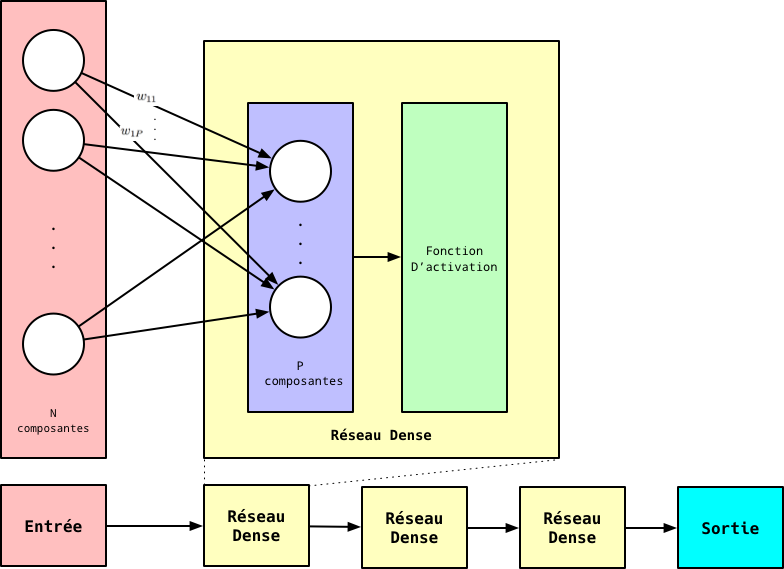
\includegraphics[scale=.3]{./assets/DeepLearning/Dense}
    \caption{Schéma d'un modèle dense et de la réalisation d'un réseau dense}
\end{center}
\end{figure}
En notant: $g^l$ pour la l ième fonction d'activation, la formule donnant la dynamique du l-ième module est: $$h^{(l)} = g^{(l)}\big(W^{(l)}h^{(l-1)} + b^{(l)} \big)$$
Les réseaux denses bien qu'extrêmment utile ont deux défaults majeurs. Le premier est l'incapcité des réseau de neurones denses à prendre en compte la temporalité. Or, dans notre cas, les actions précédent sont importantes pour déterminer l'action à effectuer. Deuxièmement, les réseaux denses ne sont pas les plus adaptés pour des tableaux de pixels (images) en entrée. Les réseaux de convolutions utilisent certaines spécificité du format image que n'utilise pas le réseau dense. Nous reviendrons sur les architectures palliant aux deux défauts cités précédemment. 

\subsubsection{Réseau de convolution et récurrent}
le réseaux de neurones à convolutions utilise l'opération de convolution pour déterminer la sortie du réseau. 
$$S(i,j) = (I * K) (i, j) = \underset{m}{\sum} \underset{n}{\sum} I(m,n) K(i-m, j-n)$$

Avec K le noyau et I l'entrée. On peut considérer l'opération de convolution comme une moyenne locale mouvante. Ainsi, elle permet d'être plus robuste aux bruits mais à de nombreux autres atouts.


Les réseaux de convolution utilisent en entrée des blocs de dimensions 3 (en pratique des tenseurs à 4 dimensions mais par simplicité, nous considerons simplement l'entrée comme un bloc 3D. On pourra penser une image RGB comme un bloc de dimension 3 dans laquelle la dernière dimension est composées des composantes bleu rouge vert). Le réseau de convolution s'est bati autour de trois idées. La première est des \textbf{intéractions locale}, ce qui veut dire que chaque entrée va intéragir avec seulement un sous ensemble de la sortie. La deuxième est le \textbf{partage des poids }, car dans le réseau a convolution, le noyau est commun à tout les pixels d'entrée (alors qu'on pourrait le changer pour chaque pixel). Cela a pour effet d'utiliser bien moins de paramètres qu'un réseau dense à taille équivalente. Enfin, troisièmment, le réseau possède \textbf{une invariance par translation}, cela implique que si un objet est translaté en sortie de réseau le résultat sera le même. Cela permet d'être plus robuste dans de nombreux cas.

Le réseau de convolution est composé d'un noyau qui est l'équivalent des poids dans le réseau de neurones denses. Il est utilisé dans l'opération de convolution. C'est le noyau qui est optimisé dans le but de minimiser une certaine fonction de coût.

\begin{figure}[h!]
\centering
\begin{minipage}{.5\textwidth}
  \centering
  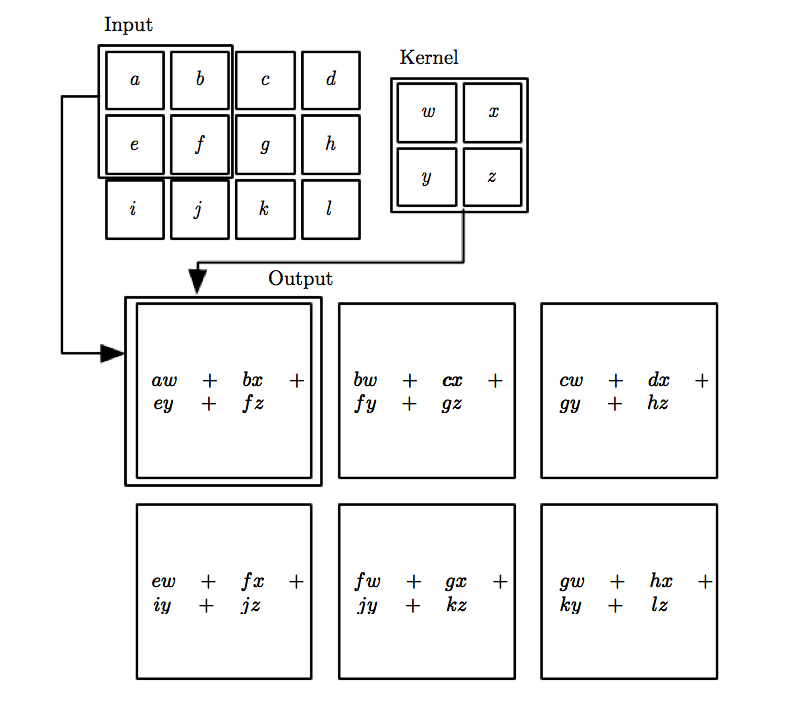
\includegraphics[width=.4\linewidth]{./assets/DeepLearning/conv.png}
  \captionof{conv}{Opération de convolution dans un CNN}
  \label{fig:test1}
\end{minipage}%
\begin{minipage}{.5\textwidth}
  \centering
  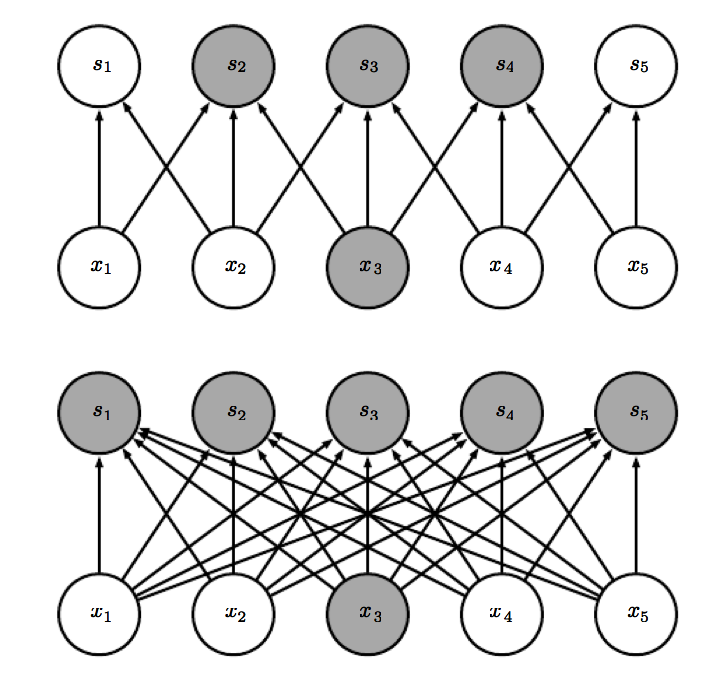
\includegraphics[width=.4\linewidth]{./assets/DeepLearning/convVSdense.png}
  \captionof{conv}{Activation de  $x_3$} 
  \label{fig:test2}
\end{minipage}
\end{figure}

Les réseaux de neurones récurrent ont été créé dans le but de pouvoir être utilisé avec des données séquentielles.
La dynamique d'un réseau récurrent est donnée pour un niveau L par la formule suivante:


\begin{gather*} 
    \left \{ \begin{tabular}{c}
            h_t = \tanh(W_{xh}x_t + W_{hh}h_{t-1} + b_h) &
            y_t = W_{hy}h_t + b_y &
    \end{tabular}
\end{gather*}

La formule ci dessous donne la dynamique du réseau récurrent le plus simple. Il souffre de nombreux problème, des alternatives existent notamment le réseau récurrent \emph{Long-Short term memory}\cite{LSTM}
. 

\begin{figure}[h!]
\begin{center}
    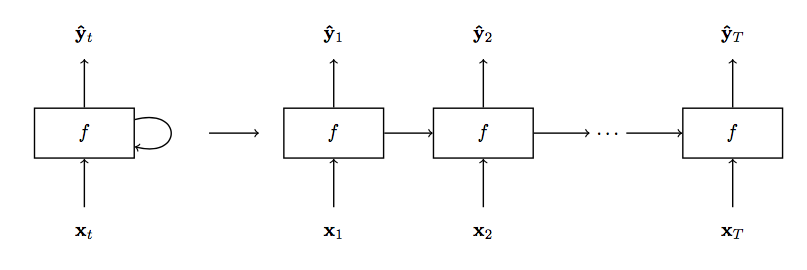
\includegraphics[scale=.5]{./assets/DeepLearning/reccurent.png}
\end{center}
\end{figure}

\subsubsection{Utilisation du deep learning dans le cadre de l'apprentissage par renforcement}

Dans la partie précédente, nous avons expliqué dans quel cadre il est pertinant d'utiliser l'apprentissage statistique (ou deep learning). Maintenant, nous allons comment intervient précisement cette technologie dans notre contrôle par apprentissage par renforcement. 

Comme nous l'avons vu, les principaux algorithmes d'apprentissage par renforcement utilise soit la fonction d'état (V), soit la fonction d'état action (Q). Ces fonctions sont une mesure de la qualité d'un état ou d'une action selon une politique. Ainsi, il joue un rôle  centrale dans le contrôle de notre agent. Plus encore, ces deux fonctions sont inconnus, et la réussite du contrôle de l'agent repose en grande partie sur notre capacité à approximer ces fonctions. Compte tenu de la complexité supposé de ces fonctions, nous avons décider d'utiliser l'apprentissage statistique car elle a montré sa capacité à apprendre des fonctions très complexe (non linéaire).

Dans la partie précédente, nous avons introduit l'apprentissage statistique supervisé (car non connaissons les sorties souhaitées). Or, dans notre cas nous serons dans un cas dit non supervisé car nous n'avons aucun signal sur lequel travaillé pour avoir la Q ou V fonction. Notre réseau devra approximer la fonction d'état avec un signal peu intéressant qui la récompense. Cela n'est pas suffisant, nous recherchons un réseau capable d'extraire d'un état qui lui est présenté les éléments qui sont suffisamment discrimant pour juger de la qualité d'une politique (via la V ou Q fonction).


Nous pouvons donc décomposer notre architecture d'apprentissage en deux partie. La première aura pour but d'extraire de l'état les élements importants pour caractériser la qualité de l'état (la V ou Q fonction). La deuxième aura pour but d'utiliser les éléments qui sont sortie de la première partie (soit des élements plus ou moins représentatif de la qualité) et devra les utiliser pour approximer la Q (ou V) fonction.


Voici une vue schématique de l'architecture réalisée dans le papier \emph{Human-level control through deep reinforcement learning}\cite{mnih-dqn-2015}

\begin{center}
    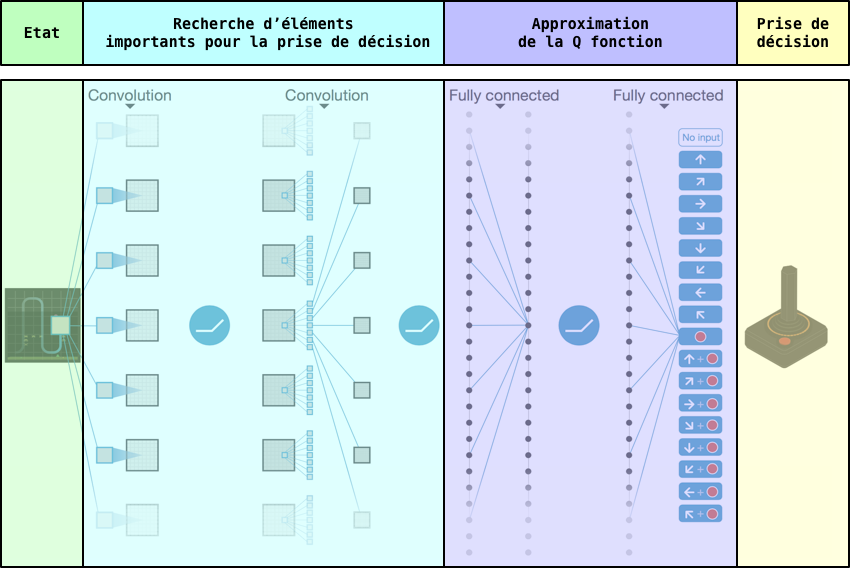
\includegraphics[scale=.5]{./assets/DeepLearning/DP_EX.png}
\end{center}
                    \newpage
\definecolor{Gray}{gray}{0.85}
\definecolor{LightCyan}{rgb}{0.88,1,1}

\section{Interface entre SE-STAR et le contrôleur}

Un grande partie de ce stage a tourné autour de l'interaction des algorithmes d'apprentissage par renforcement et SE-STAR (cf \ref{globalViewProject}). Cette partie sera consacrée à l'explication de l'architecture mise en place autour de SE-STAR pour la connection du contrôleur et de SE-STAR.
L'architecture proposée est composée de la création d'une \gls{API} simple pour communiquer avec SE-STAR et d'une interface bas niveau pour intégrer l'\gls{API} haut niveau (réalisée par Alexandre  kazmierowski).

Nous discuterons des divers difficultés que nous avons rencontré, des limites de notre architecture et des améliorations possibles.


SE-STAR est à la base un logiciel de simulation interne à THALES. SE-STAR a été prévu pour permettre une communication via l'\gls{API} de SE-STAR néanmoins le contrôle d'un seul agent par apprentissage par renforcement. Pourtant, l'API n'a pas été pensé pour un pilotae d'un agent par renforcement.  .Le contrôle des agents dans SE-STAR se base sur des stimulis internes motivationnels qui peuvent être configurés en fonction du rôle que l'on souhaite donner à un agent. Nous ne rentrerais pas dans les détails du fonctionnement original qui est complexe et orthogonal à notre objectif. Notre but est justement de créer un contrôle automatique se basant sur des stimulis extrinsèques (donnés par l'environnement) reposant sur la théorie de l'apprentissage par renforcement profond.

SE-STAR est un logiciel complexe. Il a donc fallu créer une interface  avec le contrôleur en étant le moins intrusif possible sur le code source de SE-STAR. L'objectif était de produire un code réutilisable quelques soit l'environnement. Nous nous rendrons compte que ce choix implique une perte en performance.

\begin{figure}[!h]
\centering
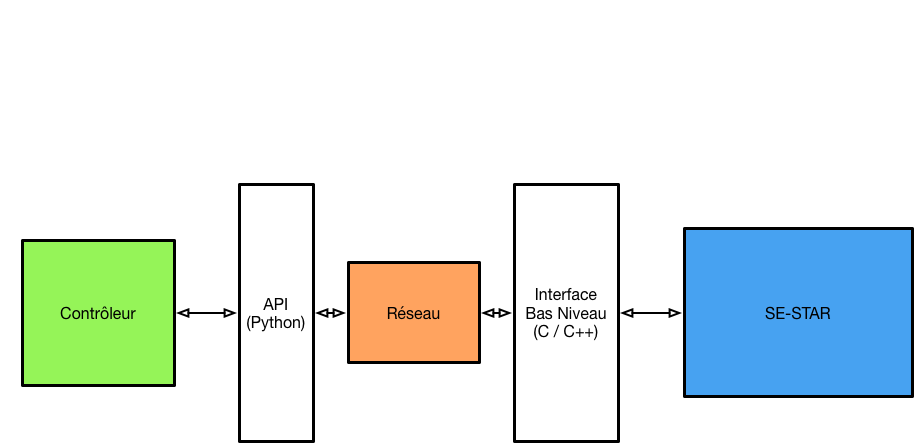
\includegraphics[width=.9\linewidth]{./assets/interfaceReseau/overviewInterface}
\caption{Vue globale de l'interaction entre le contrôleur et SE-STAR}
\end{figure}

\subsection{Analyse fonctionnelle de l'\gls{API} choisie}

Nous allons profiter de la simplicité de notre API pour l'expliquer. En apprentissage par renforcement,  un agent reçoit l'état dans lequel il se trouve. A partir de celui-ci, il interagit avec l'environnement qui lui répond en envoyant le prochain état et la récompense associée à l'état. Nous allons nous baser sur ce fonctionnement pour créer notre \gls{API}. 


\bigskip

% { --

\setlength{\arrayrulewidth}{.7mm}
\setlength{\tabcolsep}{12pt}
\renewcommand{\arraystretch}{2.}

\begin{center}
{\rowcolors{2}{white!80!gray!50}{gray!50!white!60}
\begin{tabular}{ |p{2cm}|p{8cm}|  }
\hline
\multicolumn{2}{|c|}{\gls{API} Client} \\
\hline
Fonction & Explication \\
\hline
Reset & Reset a pour but de redémarrer la simulation (obligatoire en cas de fin de partie ou si un certain temps est dépassé) \\
\hline
Step & \begin{enumerate}
\item Entrée: l'action effectuée
\item Sortie: une liste contenant l'état suivant, la récompense reçue, un booléen indiquant si la simulation est terminée et un dictionnaire donnant une multitude d'informations sur la simulation.
\end{enumerate} \\
\hline
Connect & Une fonction nous permettant d'établir une connection à distance avec un Windows distant. Nous ne parlerons pas de la méthode de connection à distance qui est assez complexe et reposant sur des outils tiers (Winexe, ...) \\
\hline
\end{tabular}
}
\end{center}

% -- May need change if set.. are not local }


L'\gls{API} est simple mais correspond exactement à la boucle classique en renforcement. Alexandre Kazmierowski a construit le serveur répondant à ces appels. L'outil créé par M. Kazmierowski permet l'interconnexion entre SE-STAR et le client .

\subsection{Principales limites et contraintes}

La simulation SE-STAR fonctionne actuellement uniquement sur Windows. Cela pose un problème car les différents outils, pour créer des algorithmes de Deep Learning, utilisent une distribution linux. Les échanges réseaux entre Linux et Windows limitent drastiquement le nombre d'images par seconde que peut recevoir l'agent (définissant la vitesse de simulation) car l'envoi d'un tableau de pixels sur le réseau est intrinsèquement coûteux. 

De plus, nous avons été confronté à de nombreux problèmes de déconnections impromptues qui ont nécessité la mise en place de mécanismes de reconnections automatiques. Néanmoins l'architecture mise en place manque encore de stabilité et n'est pas robuste à tous les types d'erreurs pouvant être rencontrés.

L'algorithme utilisé pour contrôler l'agent dans SE-STAR a été l'\gls{A3C} qui repose sur de multiples agents qui jouent dans l'environnement de façon asynchrone. Cela multiplie le nombre d'appels réseau et joue sur la stabilité de celui-ci, cela accroît la latence des appels agent (SE-STAR) / algorithme (Contrôle). De façon empirique, nous nous apercevons qu'il y a des problèmes dès que le nombre d'agents est supérieur à six. Cela s'explique en partie par le fait que SE-STAR est un logiciel demandant beaucoup de ressources, Or celui-ci n'a jamais été prévu pour une utilisation demandant de faibles ressources.Ainsi la multiplication des instances de SE-STAR peut causer des problèmes sur la machine cotée serveur si elle n'a pas assez de puissance. Alexandre  Kazmierowski nous a permis d'alléger les ressources demandées, permettant d'augmenter le nombre d'agents.

Nous pouvons dès lors nous demander si la stratégie asynchrone d'entraînement est viable.
Une problématique inhérente aux algorithmes de renforcement, qui découle de l'utilisation du deep learning, est le besoin de décorréler les états lors de l'entraînement . Or dans le cadre de nos algorithmes, cela s'avère difficile. La stratégie d'entraînement asynchrone permet la décorrélation des états lors de l'apprentissage.


En ajoutant les défaults de l'A3C, nous pouvons nous demander si d'autres algorithmes ne seraient pas plus pertinents.

\subsection{Compromis et solutions envisagées}

Dans cette partie, nous allons expliquer les solutions envisagées pour éviter de surcharger le réseau. Avant cela, il convient de revenir sur certaines contraintes sur le contrôle. En particulier, nous souhaitions avoir un contrôle qui est le moins intrusif possible sur l'environnement en l'occurrence SE-STAR.

Nous allons cependant proposer une méthode qui reste intrusive mais permet de résoudre en partie les problèmes liés à la multiplication des instances de SE-STAR et de réduire les appels réseaux. 

La méthode qui sera développée se nomme: Efficient Parallel Methods for Deep Reinforcement Learning \cite{2017arXiv170504862C}. Nous ne rentrerons pas dans les détails de l'algorithme car il est similaire à l'A3C \cite{DBLP:journals/corr/MnihBMGLHSK16}. Néanmoins,il propose une approche synchrone permettant l'utilisation du GPU. L'idée de ce papier est de proposer une architecture synchrone permettant de décorréler les états utilisés pour l'entrainement. A chaque pas, le contrôleur va décider quelles actions vont effectuer un ensemble d'agents. Le contrôleur va récupérer l'ensemble des états et des récompenses pour l'apprentissage et le choix de la nouvelle action. Quand le contrôleur rentre en phase d'apprentissage, il a un ensemble de transitions (état précédant, état actuel, action, récompense) décorrélées (car venant d'agents différents). Les premiers essais sont encourageants mais l'apprentissage n'est pas assez stable.

\begin{figure}[h!]
\begin{center}
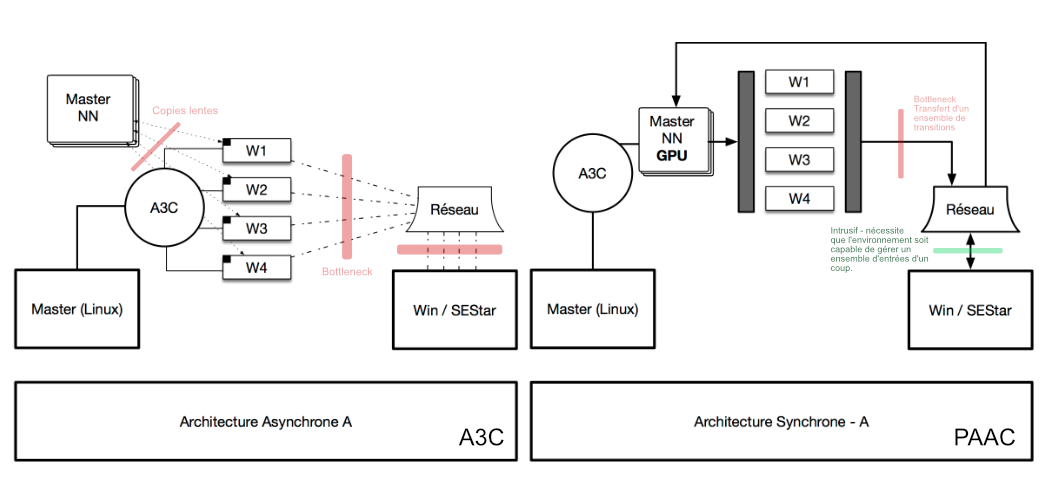
\includegraphics[scale=.4]{./assets/interfaceReseau/paaca3c}
\caption{Comparatif des algorithmes PAAC / A3C en mettant l'accent sur les problématiques réseaux}
\end{center}
\end{figure}

Nous remarquons que les principaux problèmes qui découlent de la stratégie asynchrone d'entrainement (A3C) sont liés à la communication réseau mais pas seulement. Un stratégie asynchrone exclue l'utilisation du \gls{GPU}. La stratégie synchrone de la \gls{PAAC} permet l'utilisation du GPU et impose que la simulation soit capable de gérér un ensemble d'actions en entrée. De plus, la question des transferts sur le réseau n'est pas résolue par cette approche. 

La véritable question est de savoir s'il n'existe pas d'autres approches qui suppriment la nécessité du réseau ou qui reposent sur des outils spécialement crées pour gérer les difficultés inhérentes aux réseaux. Nous verrons rapidement deux approches idéales se basant sur un outil Docker \cite{Merkel:2014:DLL:2600239.2600241} et sur l'utilisation de \gls{Wine} (qui permet de faire fonctionner des applications Windows sur Linux)

\subsection{Solutions idéales}

\subsubsection{SE-STAR sous linux via \gls{Wine}}
Notre objectif a été d'utiliser SE-STAR nativement sous Linux. Pour cela, il y a deux solutions. 
Premièrement, nous pouvons compiler directement SE-STAR pour Linux. Le problème est que le logiciel a été pensé pour une utilisation Windows et utilise des certaines librairies uniquement disponibles sur Windows. Nous ne savons pas si cela est possible même si cela aura le mérite d'être essayé. 
Deuxièmement, nous pouvons passer sous Wine pour utiliser une application Windows. Après une phase de configuration compliquée pour utiliser Wine, nous avons été en capacité d'utiliser SE-STAR sous Linux et d'utiliser l'\gls{A3C}. Nous avons remarqué des interruptions complètes de SE-STAR au bout d'une dizaine de minutes. Pour l'instant, il est difficile de savoir ce qui est responsable de ces interruptions. Nous pensons toujours que Wine est une solution viable. Il est reste néanmoins à comprendre l'origine des problèmes. Une des problématiques qui survient avec l'utilsation de Wine est que les fonctionnalités permises par SE-STAR ne sont pas entièremenet prise en charge par Wine. Cela nous oblige donc à passer par une version obsolète de Wine et possiblement moins stable.

\subsubsection{Une architecture scalable d'entrainement via Docker}
Nous allons présupposer que nous avons un moyen d'utiliser SE-STAR sous Linux. Nous exploiterons Docker (qui est un système de conteneurisation, qui groupe une application avec un environnement Linux léger configuré au préalable). Cela permet, en spécifiant les dépendances de SE-STAR, de pouvoir déployer dans un réseau n instances de SE-STAR et de simplement utilser le \emph{swarm mode} de docker pour avoir une gestion du réseau (load balancing, ...). Nous  pourrions imaginer déployer dans un cluster de cpu (ou gpu) plus de 1000 instances de SE-STAR gérées par le swarm mode de Docker. Ce genre d'architecture a déjà été utilisée.Cela pourra être mis en place dès que SE-STAR sera disponible sous Linux.

\begin{center}
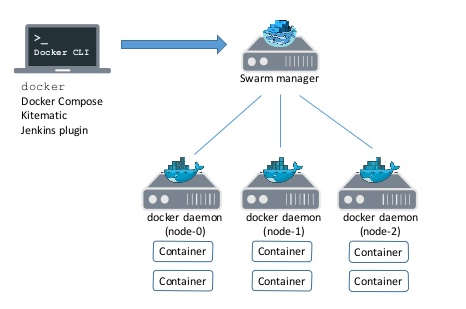
\includegraphics[scale=.5]{./assets/interfaceReseau/docker}
\captionof{figure}{Simple vue d'ensemble de l'utilisation de Docker en swarm mode}
\end{center}


Le swarm mode de Docker est une architecture composée d'un (ou plusieurs) noeud manageur qui a pour but de contrôler les noeuds enfants, de gérer le load balancing, la gestion des erreurs des noeuds enfants ... En ayant des conteneurs avec les dépendances requises par SE-STAR et l'application SE-STAR dans chaque conteneurs enfants, cela permet d'utiliser les algorithmes classiques d'apprentissage par renforcement profond à un échelle industrielle.

\subsection{Conclusion sur les questions d'interfaces et de réseaux}

A travers ce chapitre, j'ai essayé de vous expliquer les principaux enjeux dans le cadre de l'interface entre SE-STAR et les algorithmes d'apprentissage. Sur des cas jouets, ces problématiques ne font pas surfaces néanmoins, dans des applications industrielles nous sommes obligé de réfléchir à l'architecture dans laquelle nous allons déployer nos algorithmes et nos applications. Or, les \gls{frameworks} d'apprentissage et les applications peuvent être destinées à des environnements différents ou pire avoir des dépendances contradictoires. Il est donc essentiel  d'utiliser des applications capables d'isoler une application afin que celle-ci puisse être  disponible sur le réseau dans le but de pouvoir permettre la communication entre les applications.

Ci-dessous, un schéma récapitulatif de l'architecture idéal (qui a été partiellement mise en place durant le stage).


\begin{center}
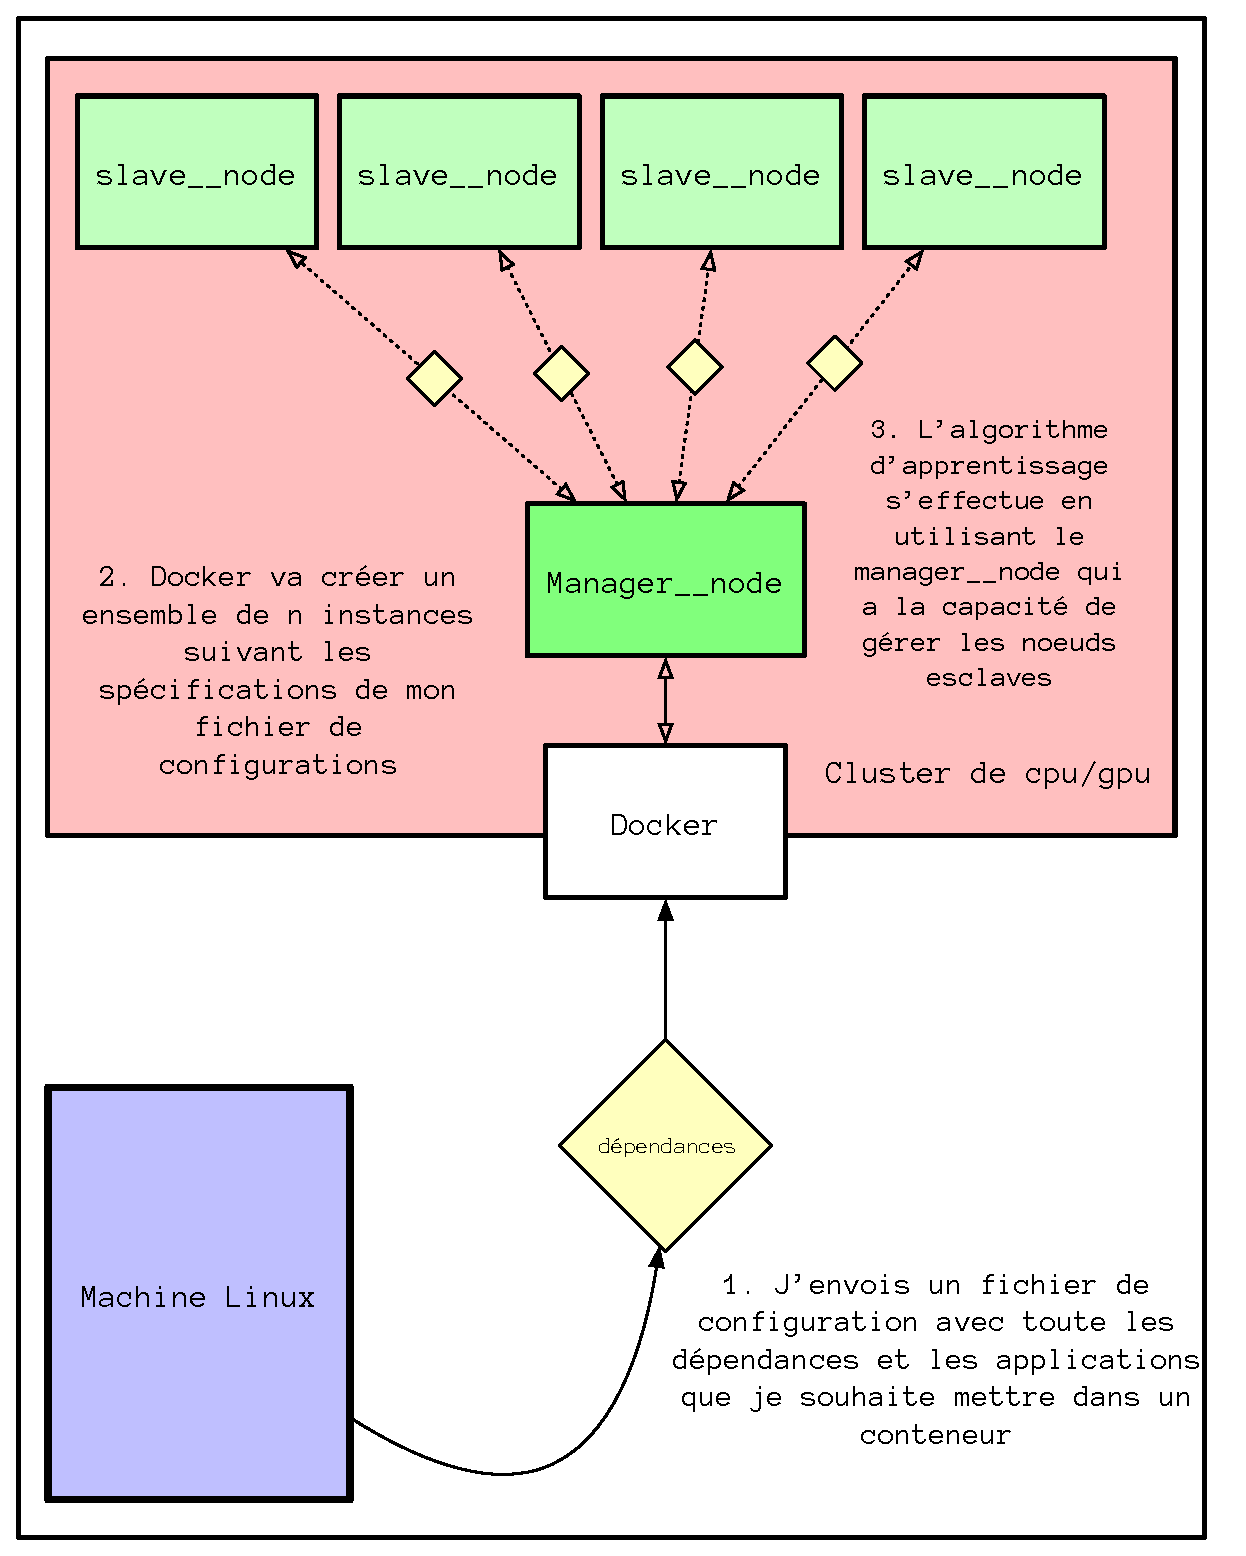
\includegraphics[scale=.7]{./assets/interfaceReseau/interfaceResume.eps}
\captionof{figure}{Vue d'ensemble de l'architecture partiellement mise en place dans le cadre de l'apprentissage de l'algorithme}
\end{center}
               \newpage
\section{Contrôle d'un agent via la simulation SE-STAR par renforcement profond}

Cette partie sera consacrée au fonctionnement du contrôle appliqué à SE-STAR. Dans le but de comprendre les choix entrepris, nous commencerons par expliquer comment fonctionne l'algorithme d'apprentissage par renforcement utilisé pour SE-STAR. Puis, nous expliquerons les faiblesses de cet algorithme (dans le contexte de SE-STAR). Enfin, nous introduirons un module de curiosité qui a pour but d'améliorer l'apprentissage et donc le contrôle de l'agent.


Nous considérons SE-STAR comme un environnement sans faire mention des problématiques liées à l'interface contrôleur / SE-STAR, ou des problématiques liés aux réseaux qui ont été développé dans la partie précédente. 

\subsection{Le choix d'un algorithme efficace pour le contrôle d'un agent dans SE-STAR.}

Il existe dans la littérature un panel très large d'algorithmes qui sont potentiellement puissants. Or, pour des questions de temps, nous n'avons pas été capable d'essayer tous les algorithmes. Nous avons donc dû faire un choix. 

Nous allons à travers cette partie, donner les principaux réseaux qui nous ont poussé à nous diriger vers un apprentissage par renforcement profond. 

Tout d'abord, les spécificités de SE-STAR impliquent le non-usage des algorihtmes \emph{model based} (basés sur un modèle, soit la connaissance de la fonction de transition). Or, il est évident que dans le cas de SE-STAR, cette fonction est inconnue. Nous pouvons même aller plus loin, la fonction de transition dans le cas d'états sous forme d'un tableau de pixels est bien souvent insoluble. Cela reviendrai à avoir la connaissance d'une fonction qui, sachant l'etat courant et l'action donne la probabilité d'être dans un nouvel état. Voici le cheminement pour déterminer le nombre de combinaisons possibles d'états pour une image de 82x82 pixels. Un pixel est composé de trois nombres de 0 à 255. Chaque pixel a la capacité de produire théoriquement $256^3 = 16\ 777\ 216\ \text{couleurs}$. Ainsi, il y a $82 * 82 * 256^3 = 112\ 810\ 000\ 384 \text{ combinaisons d'images différentes possibles}$. Nous comprenons vite l'impossibilité d'utiliser un algorithme basé sur la fonction de transition. Malgré le fait que pendant ce stage nous n'avons pas utilisé d'algorithmes purement \emph{model based}, nous pourrions toujours approximer cette fonction en utilisant une architecture de Deep Learning et en trouvant une fonction de perte adéquate.Cela est possible, mais ne sera pas testé durant ce stage car l'approche \emph{model based} est difficilement applicable dans le cas d'états sous forme de pixels (nous passons toujours par une phase de compression de l'état pour permettre ce genre d'algorithmes). Il y a peu d'algorithmes suivant ce principe qui ont montré de bon résultats sur des environnements difficiles.

\begin{itemize}
    \item Notre algorithme d'apprentissage par renforcement appartiendra à la famille des \textbf{algorithmes sans modèle (\emph{Model Free})}
\end{itemize}

Il existe beaucoup d'algorithmes dans la famille \emph{Model Free}. Nous souhaitons donc utiliser en premier lieu un algorithme qui est robuste et performant selon la littérature. De plus, nous aimerions un algorithme qui soit extensible. En effet, comme nous le verrons plus tard avec le module de curiosité, la plupart des environnements 3D sont  difficiles pour les algorithmes d'apprentissage par renforcement. 

Au vue de la littérature, il y a deux méthodes qui ressortent:
\begin{enumerate}
\item \bf{Deep Q Networks (DQN} \cite{mnih-dqn-2015})
\item Asynchronous advantage critic (\bf{A3C})\footnote{Nous utiliserons A3C ou DQN dans la suite de ce rapport} \cite{DBLP:journals/corr/MnihBMGLHSK16}
\end{enumerate}

Les principes sur lesquels reposent ces deux algorithmes ont été développé précédemment dans ce rapport. Bien que nous avons testé ces deux algorithmes sur SE-STAR, nous avons déjà commencé par comparer ces deux algorithmes sur des cas plus simples. Néanmois, il est à noter que sur les expérimentations, que nous avons effectué, ont été utilisées des versions améliorées du DQN de l'A3C (non indiquées dans ce rapport). En effet, ces méthodes ont trouvé un echo dans la communauté scientifique et ont été améliorées de nombreuses manières. Il serait trop long d'expliciter toutes les améliorations existantes pour ces algorithmes mais nous allons tout de même les citer et donner une référence pour les lecteurs les plus curieux.

% { -- GLOBAL CHANGE [[WARNING]]

\setlength{\arrayrulewidth}{.45mm}
\setlength{\tabcolsep}{12pt}
\renewcommand{\arraystretch}{2.}

\begin{center}
{\rowcolors{2}{white!80!gray!50}{gray!50!white!60}
\begin{tabular}{ |p{3.3cm}|p{11cm}|  }
\hline
\multicolumn{2}{|c|}{Algorithmes testés pendant le stage} \\
\hline
\multicolumn{2}{|c|}{\bf{Améliorations du Deep-Q-Network}} \\
\hline 
\textbf{Double-Q-Learning} (DDQN \cite{DDQN}) & Résout un problème intrinsèque du Deep Q Network qui est l'introduction d'un biais au niveau de l'estimation de la fonction d'état action.\\\hline


\textbf{Dueling-Q-Learning} \: (D-DQN\cite{DUEL}) & Au lieu d'approximer la fonction d'état action ($\rightarrow$ DQN), nous préférons approximer \emph{la fonction d'avantage} qui se défini comme la différence de la fonction d'état et de la fonction d'état action. Cela a de nombreuses qualités car la fonction avantage permet de déterminer si une action mène à un gain positif par rapport à la moyenne des gains espérée ce qui est plus utile que simplement la fonction d'état action dans le cadre du contrôle (la fonction avantage donne une information plus fine et intéressante que la fonction d'état action )  \\\hline

\textbf{Prioritized Replay}\cite{REPLAY} & Pour décoreller l'entraînement dans le cadre de l'apprentissage  en utilisant le DQN, nous sommes obligé de nous servir d'une mémoire pour stocker des transitions et pouvoir ensuite échantillonner celles-ci. La méthode de \emph{favorisation de la mémoire} consiste à échantillonner les transitions qui ont mené à la plus forte erreur (cf fonction de perte), ce qui correspond à des cas particulièrement intéressants dans le cadre de l'apprentissage.  \\\hline

\multicolumn{2}{|c|}{\bf{Améliorations de l'A3C}} \\
\hline 

\textbf{GAE}\footnote{Generalized Advantage Estimation tiré du papier: High-Dimensional Continuous Control Using Generalized Advantage Estimation }\cite{GAE} & La méthode GAE (voir note de bas de page pour avoir la référence) est une méthode qui n'est pas directement affiliée à l'A3C mais qui a été utilisée dans celle-ci et est devenu quasiment standard. L'idée est d'utiliser un estimateur de la fonction d'avantage qui est biaisé mais qui possède une variance plus faible. Il a été montré empiriquement que son utilisation améliore grandement l'apprentissage. \\\hline
\textbf{UNREAL}& A3C-GAE avec en plus des objectifs auxiliaires pour améliorer la stabilité du réseau et pousser l'agent à explorer son environnement.
\\\hline
\end{tabular}
}
\end{center}


Comparons empiriquement les méthodes dérivées du DQN et de l'A3C.

\subsection{Comparaison entre les méthodes issues de la famille du DQN et de l'A3C}

\subsubsection{Les algorithmes issus de la famille du Deep Q Learning}

% TODO -------------------------

Les résultats sont issus d'expérimentations sur l'environnement de contrôle cartpole, où le but est de maintenir une barre sur un ensemble mobile le plus longtemps possible. L'ensembles des actions est composé de LEFT pour aller à gauche et RIGHT  pour aller à droite. L'agent reçoit une récompense de +1 à chaque pas de temps. L'environnement est réussi lorsque que l'agent a 200 points (nombre de points maximum).

\begin{center}
    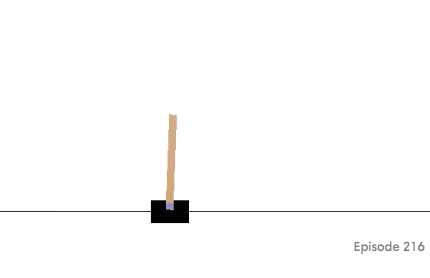
\includegraphics[scale=.5]{./assets/DeepLearning/cartpole.png}
\end{center}

\begin{figure}[H]

\begin{minipage}{.5\linewidth}
\centering
\subfloat[]{\label{main:a}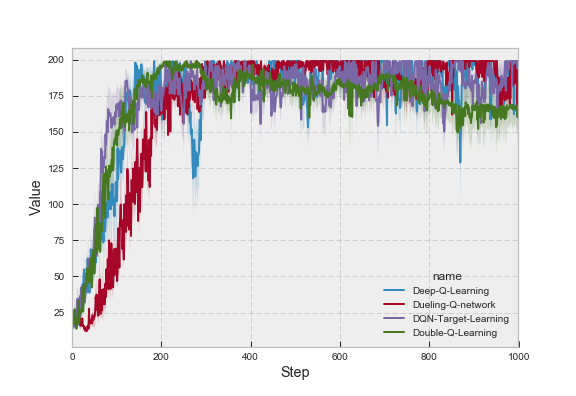
\includegraphics[width=1\linewidth]{./assets/DQNResult/4}}
\end{minipage}%
\begin{minipage}{.5\linewidth}
\centering
\subfloat[]{\label{main:b}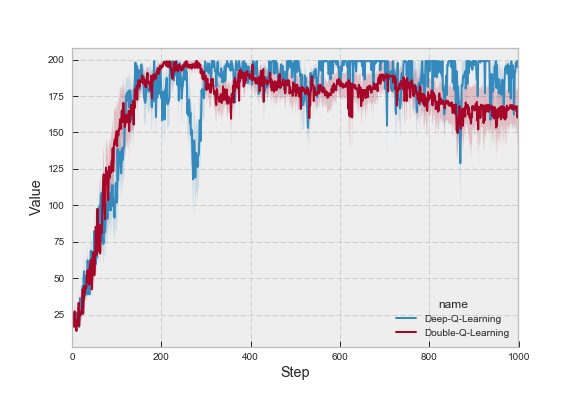
\includegraphics[width=1\linewidth]{./assets/DQNResult/2}}
\end{minipage}\par\medskip

\begin{minipage}{.5\linewidth}
\centering
\subfloat[]{\label{main:a}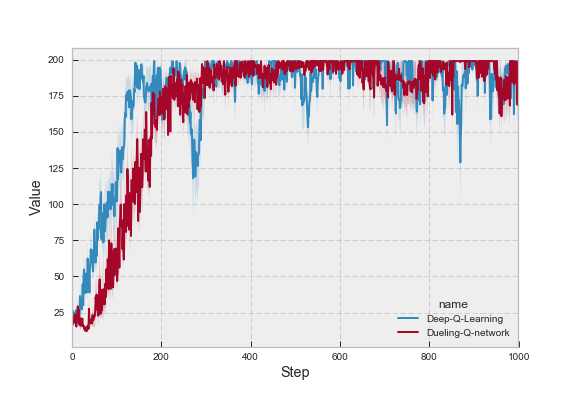
\includegraphics[width=1\linewidth]{./assets/DQNResult/3}}
\end{minipage}%
\begin{minipage}{.5\linewidth}
\centering
\subfloat[]{\label{main:b}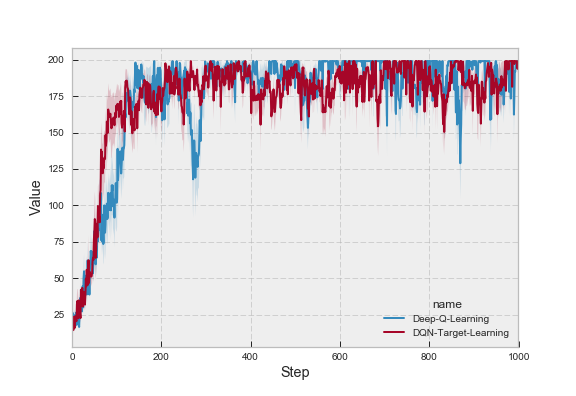
\includegraphics[width=1\linewidth]{./assets/DQNResult/1}}
\end{minipage}\par\medskip
\caption{Résultats du Deep Q learning sur CartPole}
\label{fig:main}
\end{figure}

A travers ces premiers résultats, nous pouvons comparer les différents algorithmes issues de la famille du Q Learning.

Nous pouvons remarquer que, quelque soit l'algorithme issu de la fammile du Q Learning, l'apprentissage est dans l'ensemble stable. En effet, Nous ne voyons pas, pour la majorité des algorithmes testés,  de chutes de performance durant l'apprentissage. Cependant, il y a de faibles différences concernant la dynamique d'apprentissage. L'algorithme le plus simple (\emph{le Deep-Q-Learning} a la dynamique la plus rapide pour arriver de façon quasiment stable à 200 points avec le Deep-Target-Learning\footnote{une version du DQN visant à stabiliser l'apprentissage}}. Ceci s'explique car les dérivés du DQN stabilisent l'entraînement au prix d'un apprentissage plus long. 
Il est à noter que tous les autres algorihtmes issus du Q learning ont été testés dans la version avec \emph{Target}. Nous pouvons ainsi voir que, globalement, le DQN est un peu moins stable que les autres algorithmes (présence de pics avec un score faible). Enfin, nous pouvons constater que \emph{le dueling-Q-network} et le DQN avec target sont les plus stables et donc les plus adéquats.

Ce constat est corrélé avec d'autres expérimentations faites qui ne sont pas présentent dans ce rapport.


\subsubsection{Les algorithmes issus de la famille de l'A3C}

\begin{figure}[h]

\begin{minipage}{.5\linewidth}
\centering
\subfloat[]{\label{main:a}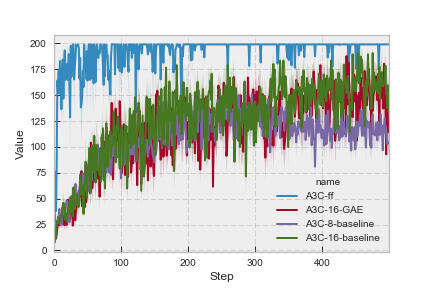
\includegraphics[width=1\linewidth]{./assets/A3CResult/11}}
\end{minipage}%
\begin{minipage}{.5\linewidth}
\centering
\subfloat[]{\label{main:b}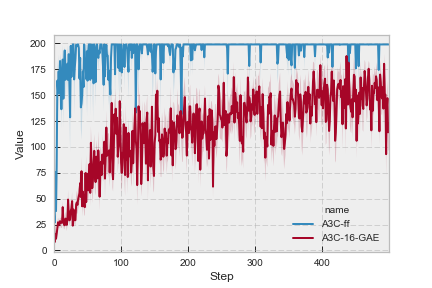
\includegraphics[width=1\linewidth]{./assets/A3CResult/22}}
\end{minipage}\par\medskip

\begin{minipage}{.5\linewidth}
\centering
\subfloat[]{\label{main:a}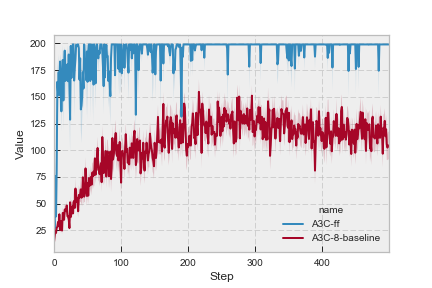
\includegraphics[width=1\linewidth]{./assets/A3CResult/33}}
\end{minipage}%
\begin{minipage}{.5\linewidth}
\centering
\subfloat[]{\label{main:b}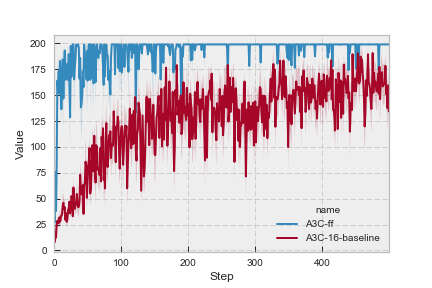
\includegraphics[width=1\linewidth]{./assets/A3CResult/44}}
\end{minipage}\par\medskip

\caption{Résultats de l'A3C sur CartPole}
\label{fig:main}
\end{figure}

Nous avons réalisé les mêmes expérimentations avec des algorithmes issus de la famille de l'A3C. Nous avons testé en particulier deux variantes de l'A3C.
\begin{itemize}
    \item A3C-FF \\
        Pour A3C Feedforward, cela fait référence au type de réseau de neurones utilisé en sortie du réseau de convolution. En particulier, le réseau de neurones correspond au modèle ldense précédement décrit.
    \item A3C-LSTM \\
        LSTM correspond à un réseau de neurones récurrent qui a la particularité par rapport au réseau dense de prendre en compte les états précédents. Ce type de réseau est pertinant dans le cas où nous avons seulement une image partielle de l'environnement.
\end{itemize}
De plus, nous avons comparé ces types d'algorithmes avec un nombre différent de processus. Rappelons que l'A3C est un algorithme asynchrone se basant sur de multiples agents (dans la littérature entre 4 et 32 processus sont habituellement utilisés) 
Nous remarquons que l'A3C est quasiment deux fois plus rapide que le DQN (et ses variantes) pour arriver au score maximum de 200 points dans sa verison Feedforward (FF). Cela s'explique car un réseau récurrent est bien plus long à entrainer. Pour des applications complexes nous préférerons la version LSTM de l'A3C. Ainsi, dans le cadre de SE-STAR, nous utiliserons la version LSTM.

Le nombre de processus est aussi déterminant dans la dynamique d'apprentissage. En regardant la figure c qui compare la version FF avec 16 processus (en bleu) et la version avec 8 processus, nous nous rendons compte qu'un nombre élevé de processus est bénéfique pour l'entraînement.

Cartpole est un environnement relativement simple à résoudre. L'environnement est éloigné de notre cas d'usage qui sera SE-STAR. Nous avons donc testé les différents algorithmes sur des environnements plus complexes. 
Ci dessous, les résultats pour différents environnements 2D dans lesquels l'état est un tableau de pixels (82*82). Ces environnements sont plus complexes que Cartpole pour au moins trois raisons. 
La première est qu'il y a un nombre élevé d'actions (douze en moyenne), la deuxième est que l'état possède une haute dimensionnalité. Enfin, les récompenses sont données seulement à la fin d'un épisode ou  plus rarement que dans Cartpole. Cela ralenti l'entraînement assez fortement et posera de nombreux problèmes.  


\begin{figure}[H]

\begin{minipage}{.5\linewidth}
\centering
\subfloat[]{\label{AAA}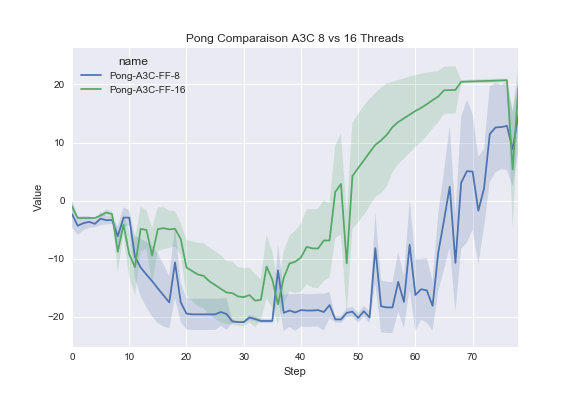
\includegraphics[width=1\linewidth]{./assets/ATARI_RESULT/pong.png}}
\end{minipage}%
\begin{minipage}{.5\linewidth}
\centering
\subfloat[]{\label{BBB}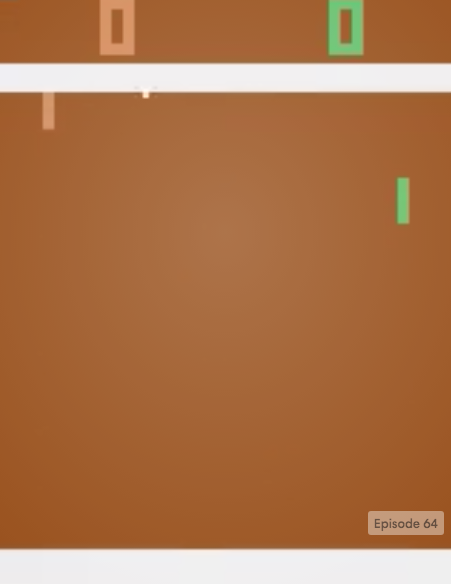
\includegraphics[width=.6\linewidth]{./assets/ATARI_RESULT/pong1.png}}
\end{minipage}\par\medskip

\begin{minipage}{.5\linewidth}
\centering
\subfloat[]{\label{main:Seaquest}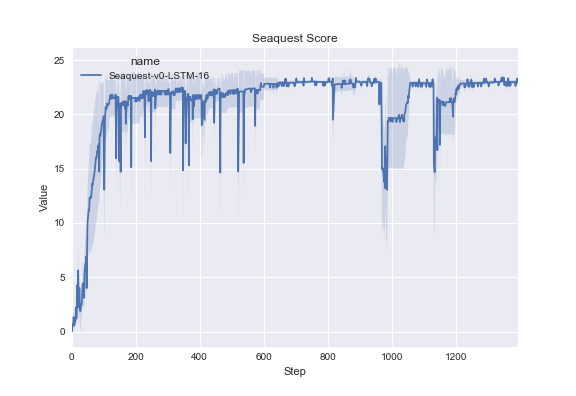
\includegraphics[width=1\linewidth]{./assets/ATARI_RESULT/Seaquest.png}}
\end{minipage}%
\begin{minipage}{.5\linewidth}
\centering
\subfloat[]{\label{main:b}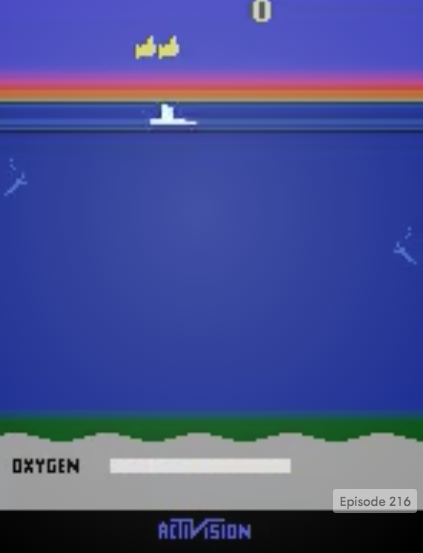
\includegraphics[width=.6\linewidth]{./assets/ATARI_RESULT/Sequest1.png}}
\end{minipage}\par\medskip


\begin{minipage}{.5\linewidth}
\centering
\subfloat[]{\label{main:a}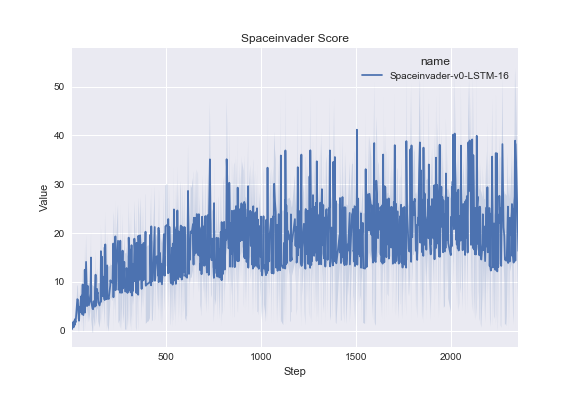
\includegraphics[width=1\linewidth]{./assets/ATARI_RESULT/Spaceinvader.png}}
\end{minipage}%
\begin{minipage}{.5\linewidth}
\centering
\subfloat[]{\label{main:b}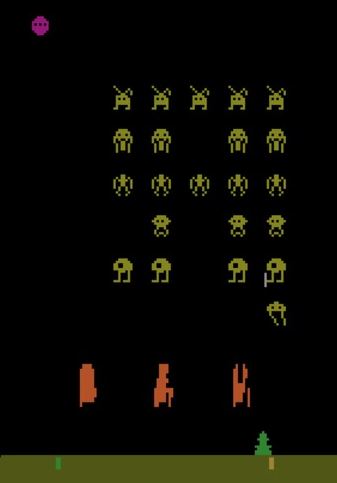
\includegraphics[width=.6\linewidth]{./assets/ATARI_RESULT/Spaceinvader1.png}}
\end{minipage}\par\medskip


\caption{Résultats de l'A3C sur des environnements ATARI}
\label{fig:main}
\end{figure}

Nous avons utilisé l'A3C-LSTM-GAE pour l'apprentissage car il a montré de meilleurs résultats d'après nos tests. Nous n'avons pas utilisé un algorithme issu de la famille du Q-Learning car un des défault de cette famille est la lenteur pour converger vers une bonne politique. Nous avons déjà mentionner qu'intrinsèquement le Deep-Q-Learning avait des problèmes de stabilité, or les stratégies pour le stabiliser ont aussi pour effet d'entraver la dynamique d'apprentissage de celui-ci. Dans la suite de ce rapport, nous privilégierons donc les méthodes se basant sur la famille de l'A3C.

\subsection{Spécification des différents environnements créés par SE-STAR}

Dans cette partie, nous introduirons les environnements qui ont été utilisés avec notre architecture de contrôle. Nous avons créé plusieurs environnements et plusieurs représentations (images 2D vue de haut, vue FPS\footnote{Vue classique des jeux vidéo d'action, où l'on voit seulement ce que l'agent voit}). Nous montrerons qu' à l'heure actuelle, certains environnements sont difficiles à utiliser avec de l'apprentissage par renforcement pour des raisons que nous verrons ultérieurement.

\subsubsection{Environnement labyrinthique simple créé par SE-STAR}

L'objectif de ce stage fut de contrôler un agent à travers un environnement labyrinthique dans le but de trouver la sortie de celui-ci. Notre premier environnement fut extrêmment simple. 

Ci-dessous, une image de l'environnement créé et de la representation associée à celui-ci.


\begin{figure}[h!]
\centering
\begin{minipage}{.5\textwidth}
  \centering
  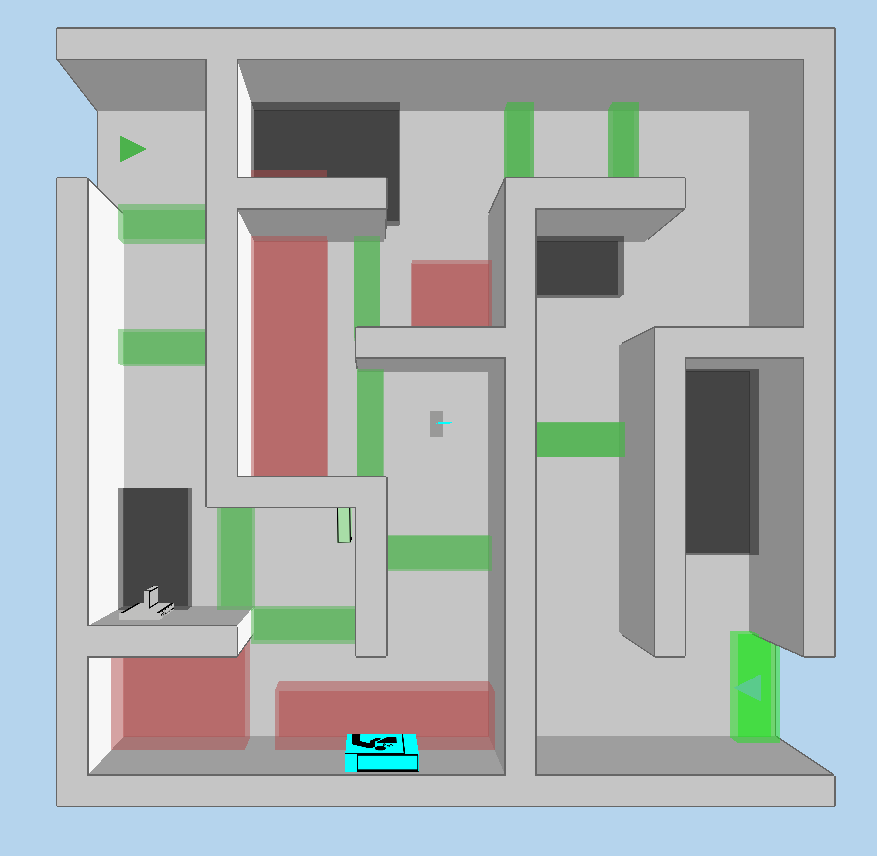
\includegraphics[width=.5\linewidth]{./assets/SESTAR/env_sestar_agent.png}
  \caption{Environnement A en 3D}
  \label{fig:test1}
\end{minipage}%
\begin{minipage}{.5\textwidth}
  \centering
  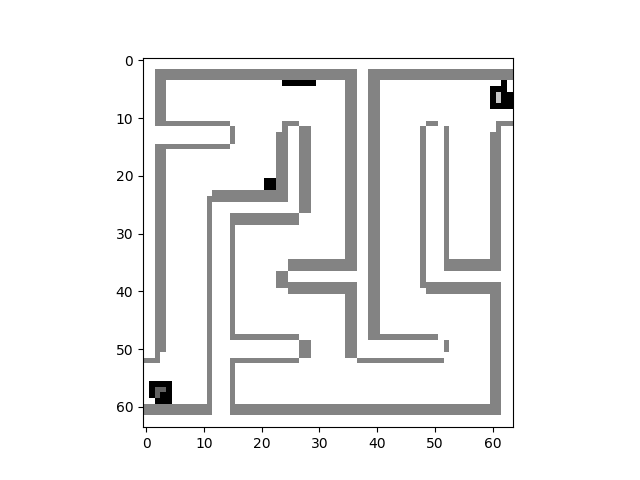
\includegraphics[width=.65\linewidth]{./assets/SESTAR/vue_agent_1.png}
  \caption{\small{Environnement A par l'agent}}
  \label{fig:test2}
\end{minipage}
\end{figure}

\todo[inline]{Transformer en tiré ou tableau}
Nous pouvons voir en rouge les coins où l'agent va recevoir une pénalité de -0.1, et en vert foncés les coins où l'agent va recevoir une récompense de +0.1. Le coin en vert clair représente l'arrivé souhaitée (avec une récompense de +1). Les lieux en noir sont des lieux où l'agent est très fortement pénalisé (par une pénalité de -1) et une interruption de l'environnement (équivalent à un game over\footnote{partie perdue dans un jeux video}). Quand l'agent passe dans une zone où il reçoit une récompense, toute la zone disparait pour éviter des stratégies où l'agent tournerait en rond dans une zone à récompenses. 

Ci-dessous un tableau récapitulatif des spécifications de l'environnement:


\rowcolors{2}{blue!10}{blue!25}
\begin{center}
    \begin{tabular}{|c|c|}
    \Xhline{2\arrayrulewidth}
    \multicolumn{2}{|c|}{Spécifications} \\
    \Xhline{2\arrayrulewidth}
    Gestion des actions & De 4 à 9 actions (modulables) \footnotemark\\
    Durée des actions & Quatres pas de temps \\
    Format de l'état&2D\\
    Taille de l'image & 42 * 42\\
    Prise en compte de l'orientation& Oui\footnotemark\\
    \Xhline{2\arrayrulewidth}
\end{tabular}
\end{center}
\footnotetext{On utilisera les actions suivantes: HAUT, BAS, DROITE, GAUCHE, DIAGONALES (4 actions), et NO-OP (ne rien faire)}

\footnotetext{Les actions ont un effet différent en fonction de l'orientation}

Nous avons noté un apprentissage très difficile avec ce type d'environnement. Cela est principalement dû à des problèmes réseaux qui ont ralenti et complexifié l'entraînement. Néanmoins, nous avons noté que l'état donné à l'agent était difficilement exploitable. Un problème avec la représentation qu'on a adopté (en 2D) est l'absence de vision du placement des récompenses. Or, comme nous l'avons déjà noté, pour réussir un apprentissage, l'agent doit être capable de récupérer des informations pertinantes de l'état. Cela n'est pas possible avec la représentation actuelle.

Nous avons donc utilisé le même environnement avec une représentation. Ci-dessous, la véritable image sortie du simulateur et l'image donnée à l'agent pour l'apprentissage.

\begin{figure}[h!]
    \begin{center}
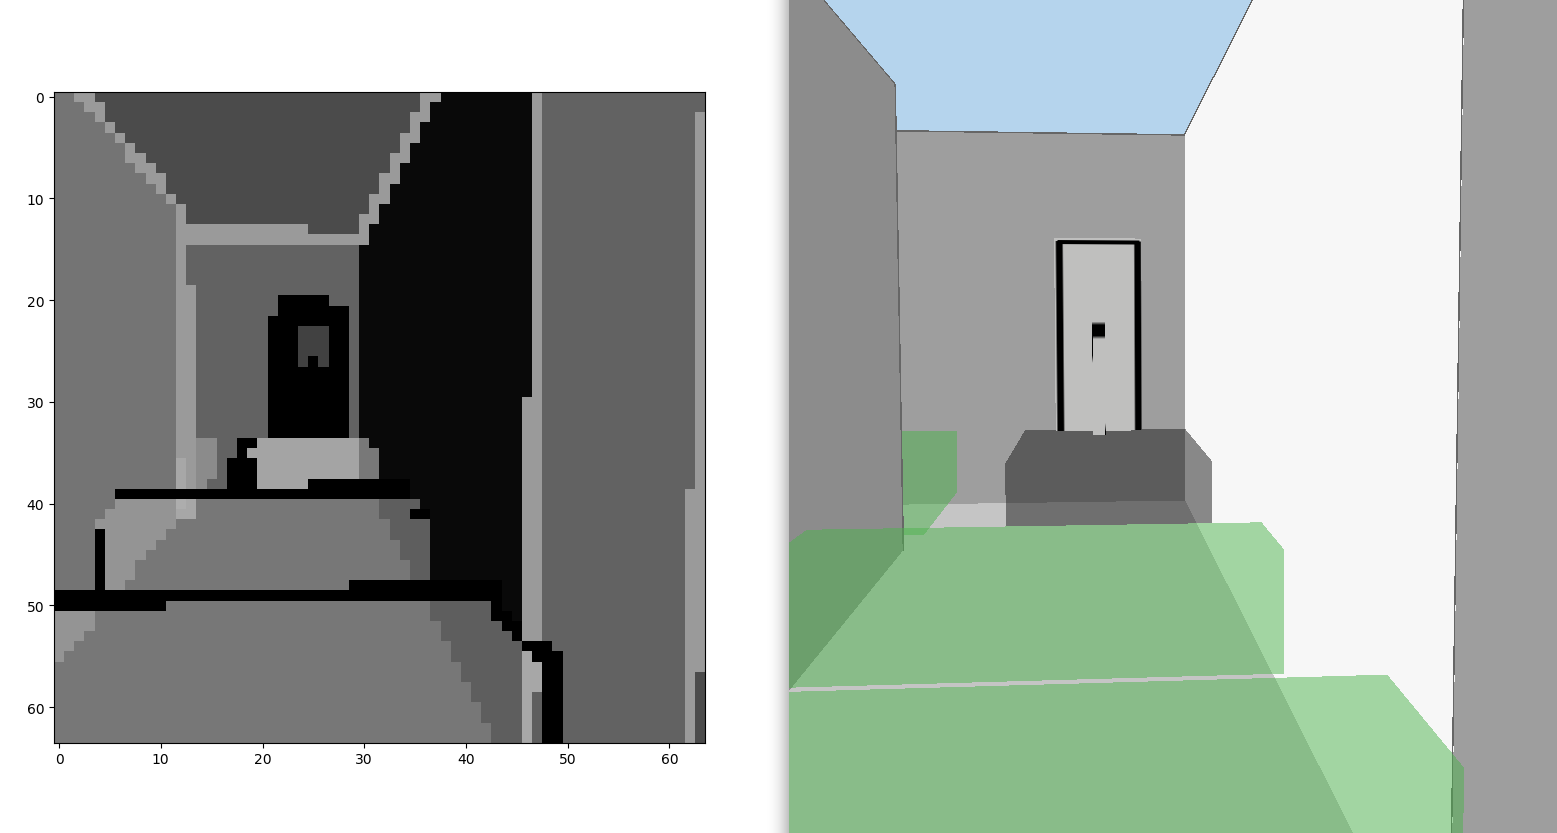
\includegraphics[scale=.15]{./assets/SESTAR/se2.png}
\caption{Représentation 3D de l'environnement}
\end{center}
\end{figure}

Comme le montre les figures au dessus, la vue est partielle et correspond à ce que voit l'agent. Les zones de récompenses sont maintenant visibles mais le résultat n'est pas satisfaisant. En effet, avec la nouvelle représentation qui est une vue 2D partielle est particulièrement difficile pour notre agent. Les environnements 3D avec une vue 2D donnés à un agent sont complexes pour des agents entraintés via A3C (ou DQN). Cela s'explique car ce genre d'algorithmes utilise une architecture qui cherche des éléments saillants dans l'environnement pour pouvoir approximer la Q fonction et trouver la politique optimale. Or dans notre environnement il y a peu d'élements possiblement interessants pour approximer la Q fonction. De plus, la Q fonction (ou fonction d'état-action) donne une estimation de la valeur d'une action suivant une politque. Le problème est que nous utilisons des actions qui dépendent fortement de l'orientation de l'agent. Si l'agent choisit d'avancer, selon l'orientation de celui-ci, l'action AVANCER aura un sens radicalement différent du point de vuede l'agent. Cela implique que l'approximation recherchée est quasiment impossible.


Pour régler un maximum de problèmes, nous avons créé  un environnement similaire qui possède plus d'éléments caractéristiques  pour aider l'agent. Nous avons supprimé la dépendance par rapport à l'orientation de l'agent. 


\begin{figure}[h!]
    \begin{center}
        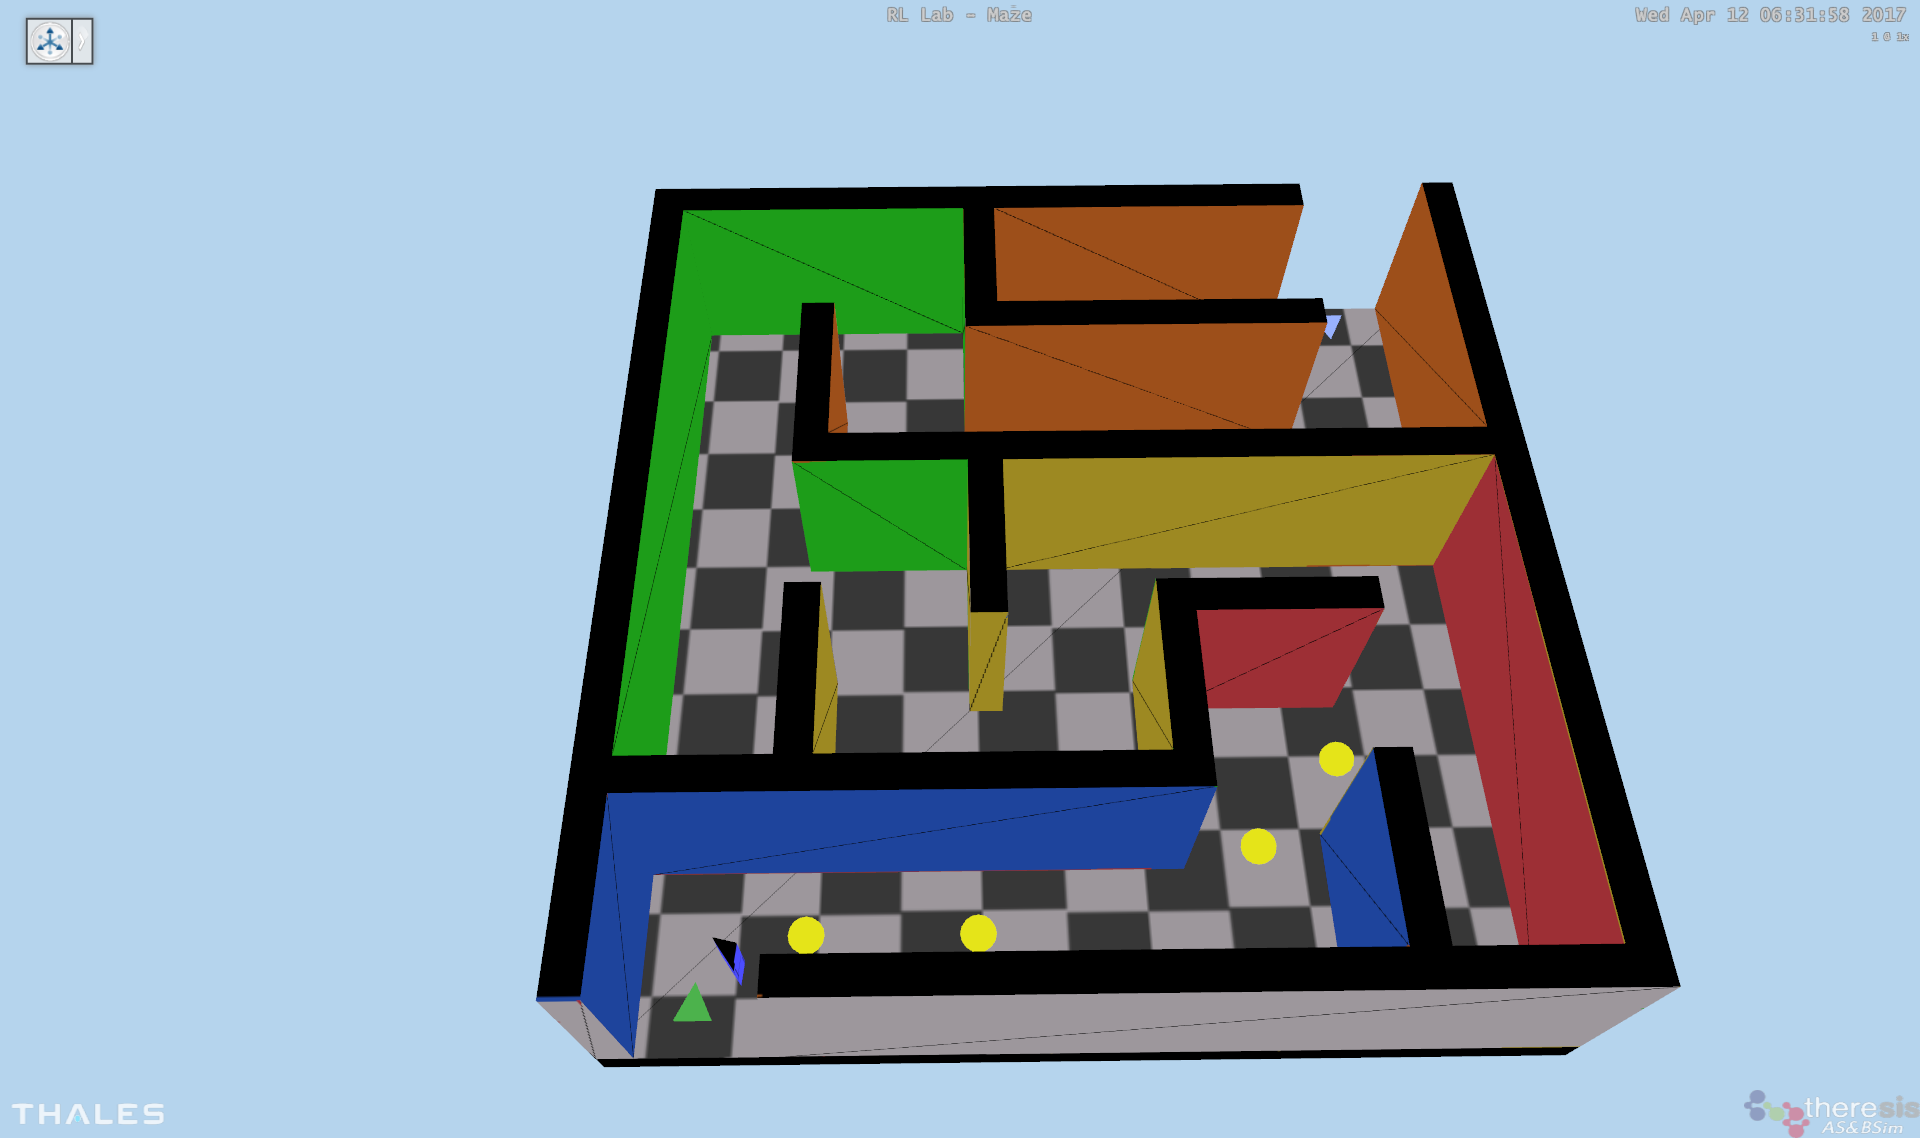
\includegraphics[scale=.15]{./assets/SESTAR/env_sestar_color.png}
\caption{Représentation 3D de l'environnement B}
\end{center}
\end{figure}

Comme nous le voyons, l'environnement est plus coloré pour permettre à l'agent un apprentissage plus aisé. La spécification reste globalement la même sauf pour la dépendance par rapport à l'orientation. 

\rowcolors{2}{red!10}{red!25}
\begin{center}
    \begin{tabular}{|c|c|}
    \Xhline{2\arrayrulewidth}
    \multicolumn{2}{|c|}{Spécifications} \\
    \Xhline{2\arrayrulewidth}
    Gestion des actions &  4 actions (modulables) \footnotemark\\
    Durée des actions & Quatres pas de temps (modulables) \\
    Format de l'état&3D\\
    Taille de l'image & 42 * 42\\
    Prise en compte de l'orientation& Non \\
    \Xhline{2\arrayrulewidth}
\end{tabular}
\end{center}

Avec cet environnement, nous avons une bonne base d'expérimentation. Malheureusement, nous n'avons pas pu expérimenter autant de temps que nous l'aurions voulu. Nous avons pu démontrer avec cet environnement qu'il était possible de faire intéragir des algorithmes d'apprentissages par renforcement avec un logiciel de simulation qui n'était pas adapté à cela. Compte tenu des résultats que nous avons eu, nous avons décidé d'intégrer des mécanismes de curiosité dans notre contrôle pour permettre à l'agent d'explorer l'envrionnement de façon beaucoup plus efficace. 

Le manque d'exploration a été une difficulté majeure pour l'agent. Des stratégies utilisant des motivations auxiliaires ont été mises au point pour répondre à ce problème. Nous explorerons cette idée dans la partie suivante.


                       \newpage     
\subsection{Module de curiosité}

Notre contrôleur mis en place, notre agent avait bien du mal à atteindre la moitié de l'environnement. Il est évident que l'apprentissage dans un environnement 3D était bien plus difficile. Pour nous convaincre de la difficulté d'un apprentissage sur un environnement labyrinthique, nous avons testé notre contrôle sur l'environnement de test Vizdoom (voir TODO section ?). Même constant, il est difficile pour l'agent d'explorer l'environnement et de dépasser la moitié de la carte.

Il y a deux explications naturelles à ce manque d'exploration:

\begin{enumerate}
\item L'agent ne reçoit qu'un état partiel de l'envrionnement et qui est déformé (passage 2D / 3D). 
\item Notre algorithme de contrôle ne contient aucun mécanisme poussant l'agent à explorer son environnment. Empiriquement, l'agent tourne en rond car l'A3C-LSTM-GAE favorise une uniformisation de la distribution de la politique. Dans notre cas, cela a pour effet d'avoir un agent qui va essayer toutes les actions (droite, gauche, haut, bas), et donc tourner en rond.
\end{enumerate}

Dans cette partie, nous allons expliquer comment fonctionne le module de curiosité qui a été mis en place. Nous commencerons par introduire succintement le dilemme exploration-exploitation, les différentes solutions dans le cadre de la théorie des Bandits à plusieurs armes et nous finirons pas discuter de la possibilité d'étendre les résultats au cadre de l'apprentissage par renforcement.

\subsubsection{La théorie des bandits à plusieurs bras}

Dans la théorie des bandits à plusieurs bras, un agent a un ensemble de K actions. A chaque action est associé une distribution $P_a$ de moyenne $\mu_a$. A chaque fois que l'agent choisit l'action a, il reçoit une récompense samplée depuis la distribution $P_a$ soit $r^t_a \sim P_a$. L'objectif de l'agent est de maximiser la somme des récompenses obtenues. 

$$
    \text{Maximiser: \: } \underset{t=1}{\overset{T}{\sum}}\:r^t_{a_i} \:\: \text{avec} \:\: r^t_{a_i}\sim P_a
$$

Il y a donc un paralèlle à faire entre le contexte de la théorie des bandits et celui de l'apprentissage par renforcement. Une dès grande différences est qu'en apprentissage par renforcement la distribution des récompenses est dépendante de la séquence d'action et possiblement dépendantes du temps. 

Nous nous intéressons dans cette partie à un contexte pour simple pour illustrer théoriquement le recours à un module de curiosité.

La notion de \textbf{regret} est centrale, et est défini comme la différence entre le choix optimal des actions et le choix de l'agent ($\text{Regret} = \underset{t=1}{\overset{T}{\sum}}\: \big( r_a_*^t - r^t_{a_i} \big) $).

L'idéal serait d'avoir un algorithme minimisant le regret obtenu par l'agent (trouver l'action qui mène à obtenir le maximum de récompenses). Au début, l'agent n'a évidemment pas idée des distributions $P_a$. Pour pouvoir estimer les dites distributions, il sera obliger d'effectituer des actions plus ou moins au hasard (d'\textbf{exploration} l'espace des actions). Toute la difficulté de la théorie des bandits et de savoir comment effectuer des actions de manière à explorer leur espace et savoir quand on a assez exploré pour exploiter la connaissance des estimés des distributions. 

La litérature concernant les bandits est riche néanmoins nous souhaitons justifier l'utilisation de mécanisme de curiosité via la théorie des bandits en montrant en quoi les stratégie naive son inéfficace. Ainsi, nous nous attarderons sur quatres stratégies populaires: les méthodes \textbf{Aléatoire}, \textbf{greedy}, \bm{\epsilon}\textbf{-greedy}, et\ \textbf{UCB}.

\begin{enumerate}
\item \textbf{La sélection d'actions aléatoire.}\\
C'est la stratégie la plus simple qui consiste à aléatoirement choisir une action. Cette stratégie est inefficace pour plusieurs raisons, la plus importante est qu'elle ne prend en compte les récompenses obtenues antérieurement.
Le regret espéré avec la méthode aléatoire est égale à: $T \big(\:\mu^* - \overset{\sim}{\mu}\: \big)$. Le regret croit de manière linéaire avec cette méthode, ce qui indique l'incapacité de cette méthode à trouver l'action optimale (ce qui est évident compte tenu de la méthode)
\item \textbf{La sélection d'actions selon la méthode greedy}\\
    La méthode greedy (pour avide) est une méthode de selection qui se contente de selectionner l'action qui à l'instant t, selon l'estimation de l'agent, donne la meilleur espérence de gain (de façon plus formelle $ a = \underset{a}{\text{argmax}} Q[a]$, avec Q le gain espéré estimé). Le problème est donc que l'agent va choisir continuellement un action dès lors qu'il n'aura plus d'égalité en espérence de gain selon les actions. Or, il est fort problème que l'estimation de l'agent soit mauvaise et donc qu'il se trompe d'action optimale. Avec cette méthode, le regret espéré est de: $T \big(\:\mu^* - \overset{\sim}{\mu_{a_i'}}\: \big)$, avec $i'$ l'action choisie en premier. Sans surprise, le reget crois de manière linéaire.
\item \textbf{La sélection d'actions selon la méthode} \bm{\epsilon} \textbf{-greedy} \\
    La\ méthode\ $\epsilon$-greedy est une variante de la méthode greedy dans laquelle l'action est choisie de façon greedy avec une probabilité de 1-$\epsilon$ et de façon aléatoire avec une probabilité $\epsilon$. Nous avons une borne inférieur de regré espéré qui est de $T \epsilon \big(\:\mu^* - \overset{\sim}{\mu}\: \big)$. Dans ce cas, le regret croit aussi de manière linéaire néanmoins nous voyant que si nous pouvons faire décroitre $\epsilon$ alors il serait théoriquement possible de faire croitre le regret seulement de façon logarithmique. C'est la méthode de sélection utilisé dans le \textbf{Deep-Q-Learning} et ses variantes. 

\item \textbf{La selection d'actions selon la stratégie UCB} \\
    \gls{UCB} pour \emph{Upper-Confidence-Bound} repose sur le principe d'optimisme face à l'incertitude. Ce principe stipule que plus nous sommes incertain de notre estimation sur le gain espéré plus il faut explorer cette action. On peut montrer théoriquement que dans le contexte des bandits simples, cela correspond à choisir de façon greedy plus un facteur de motivation à l'exploration. Soit formellement: 
    $$ \text{action} = \underset{a}{\text{argmax}}\bigg[Q[a] + \text{Curiosité}\bigg]  $$
    avec $\text{Curiosité} = \sqrt\frac{2\log t}{N(a)}$. On peut montrer que le regret croit de façon logarithmique ce qui est mieux que les stratégies précédantes.
\end{enumerate}

::IMAGE RECAPITULATIF

On pourrait donc imaginer utilisé une variante de l'\gls{UCB} dans le cadre de notre projet de contrôle. Néanmois, les formules données ci dessus ne sont valables que dans le cadre restreint au bandits. 
Sans pour autant utiliser \gls{UCB}, on pourra partir de cette idée de nécessité une motivation auxiliaire poussant l'agent à explorer l'environnement. Dans la partie suivante, nous allons tacher de définir plus précisement ce que veut dire d'explorer un environnement et nous allons proposer un module de curiosité pour arriver au contrôle de notre agent.

\subsubsection{Exploration et Motivation auxiliaire}

Le besoin d'exploration vient du simple fait que pour estimer la fonction d'état (ou d'état action), il faut avoir déjà recontré l'état visé. Or, dans le cas d'un environnement où l'agent n'a accès qu'a une vue partielle de l'environnement il est difficile d'estimer ces fonctions pour chaque état. Il apparait donc nécessaire de pousser l'agent à explorer en partie l'envrionnement pour déterminer au mieux une politique. Commne nous l'avons vu, dans la partie précédente, l'utilisation d'une récompense auxiliaire poussant à explorer l'environnement à du sens. Néanmoins, dans le contexte de l'apprentissage par renforcement les stratégies du style UCB (ou Bayesienne avec le sampling de Thomson) sont difficilement réalisable.

Pourtant, ce n'est pas la seule difficulté, l'état que reçoit notre agent est une représentation partielle de l'environnement. En effet, l'agent ne voit qu'un représentation 2D d'un environnement 3D. La question est donc de savoir comment explorer à partir d'une représentation compréssée de l'état. Cette problématique est au centre de la récherche en apprentissage par renforcement. Il y a plusieurs piste envisagées.

\begin{enumerate}
    \item Objectifs secondaires aidant l'agent dans ça prise de décision. Par exemple, nous pourrions optimiser notre réseau de neurones pour qu'il maximise la réduction de profondeur ($\text{depth}_{s1} > \text{depth}_{s2}$). Le problème de cette approche est qu'elle est dépendante de l'environnement.Or l'utilisation de l'apprentissage par renforcement est intéressante car elle permet d'être applicable à un grand nombre d'environnement sans grand changement.
    \item Formaliser le concepte d'exploration de façon générique. Nous chercherons une manière d'explorer un environnement à partir d'une représentation latente (compréssée) de celui ci. Il n'y a pas de consensus sur ce sujet actuellement.

    \item Utiliser des objectifs secondaires génériques. Par exemple, si nous pouvions formaliser de manière même simpliste la notion de curiosité, on peut faire l'hypothèse aurait pour effet une amélioration des performences l'algorithme car il en découlerait une exploration.
\end{enumerate}

\begin{figure}[h!]
\begin{center}
    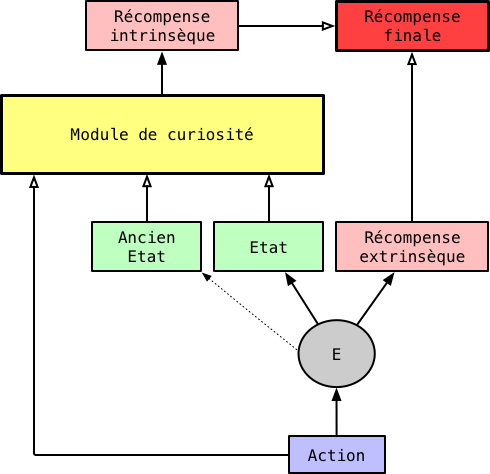
\includegraphics[scale=.5]{./assets/CURIOSITY/curiosity.png}
    \caption{Structure d'un module de curiosité}
\end{center}
\end{figure}

\subsection{Motivations auxiliaires et motivations}

Les motivations auxiliaires ont pu but d'aider l'agent à explorer son environnement. En effet, plus l'état est dimensionnelle élevée plus cela nécessite des approches particulières pour garantir que l'agent va être pousser à explorer celui-ci. Sans module auxiliaire, il est possible que l'agent reste dans un périmêtre restreint ce qui n'est pas souhaitable.

\subsubsection{Motivations auxiliaires spécifiques au environnements 3D}

Dans un premiers temps, nous allons explorer un module de curiosité simple que nous permettra d'introduire plus tard le module de curiosité qui a été integré dans le contrôle. Ce module par d'un constat simple,en poussant l'agent à changer en permanance le flux d'entrée qu'il perçoit, l'agent devra explorer l'environnement. En effet, bien souvent un manque d'exploration implique que les états que voient l'agent resteront similaire. Si l'agent recherche des états qui sont différents les uns des autres alors on peu faire l'hypothèse que l'agent sera pousser à explorer en profondeur l'environnements pour continuer de changer son flux d'entrée.

Formellement sela consiste à prendre la différence entre deux états sucessifs et considérer leurs normes comme un signal pouvant aider l'agent.

\begin{equation}
\text{récompense intrinsèque} = \lambda \: \norm{s_1 - s_2}^2 
\label{eqn:intrinsicmotivation}
\end{equation}

L'équation ~\ref{eqn:intrinsicmotivation} est trop simple pour être utiliser. En effet, prenons le cas d'un agent qui tourne en rond, alors selon l'équation \eqref{eq:simple} l'agent serait encouragé à tourner. Ce comportememt exclu donc l'utilisation de ce type d'approche naive. Nous allons décrire une méthodequi se base sur l'intuition que nous avons developpé en utilisant une approche hiérarchique. L'idée est que l'agent dévelope un mécanisme d'attention lui permettant de savoir qu'elle sous-partie de l'état est intéressante et avec laquelle on peut employer la stratégie simpliste.
Formellement cela revient à apprendre la séquence des k tel quel:

\begin{equation}\label{eqn:hierarchicalcuriosity}
    \text{récompense intrinsèque} = \tau\: \frac{\norm{h_k \odot \big[ s_t - s_{t-1} \big]}^2}{\norm{s_t - s_{t-1}  }^2} 
\end{equation}

L'équation \ref{eqn:hierarchicalcuriosity} montre comment utilisé seulement une sous partie de l'entrée pour calculer la récompense intrinsèque. Cette formule est utilisé dans le papier \emph{Feature Control as Intrinsic Motivation for Hierarchical Reinforcement Learning}\cite{hierarchicalcuriosity}
Nous ne détaillerons pas la méthode pour déterminer la séquence de k car elle est extrêmment similaire à la façon de determiner la séquence d'action à effectuer. Nous avons aussi créer une méthode qui généralise la précédente qui au lieu de choisir un k, pondère par un facteur choisi par l'agent l'ensemble des sous ensembles de l'état pour calculer la récompense intrinsèque.

Nous avions peur de déstabiliser le réseau avec ce genre de recompense, le choix des hyperparamètres ($\lambda$, $\tau$) nécessite du soin et de nombreux essais.

Les tests préliminaires ont montrés que cela ne destabilisé pas l'apprentissage, néanmoins cela mériterais plus de test pour être convaincu de cela.

\begin{figure}[h!]
    \begin{center}
        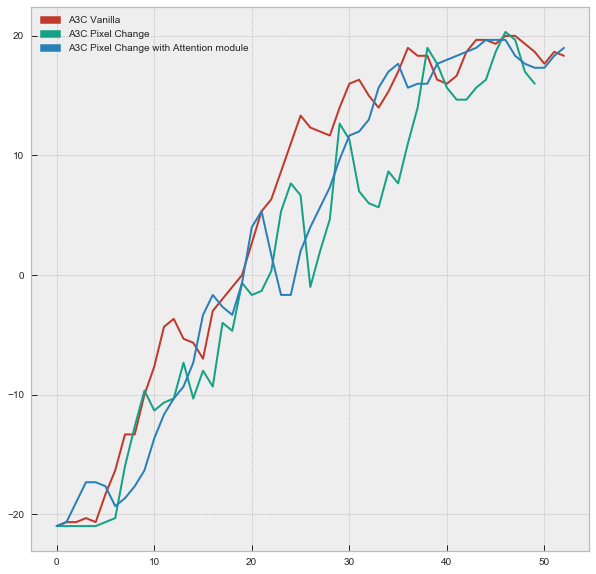
\includegraphics[scale=.35]{./assets/CURIOSITY/A3C_auxiliaire.png}
        \caption{Résultats des motivations auxiliaires sur Pong (Gym-OpenAI)}
    \end{center}
\end{figure}

Comme vous pouvez le voir le module a été testé avec comme contrôleur l'A3C. Les résultats indiquent que la recherche de la séquence de k pour un cas simple (Pong) n'augmente pas significativement l'entrainement. Il est reste maintenant a testé ce module avec SE-STAR. Les premiers résultats du contrôleur ne sont pas disponible avec ce module, il est noté que ce type de module n'a jamais été utilisé dans un cas aussi complexe qu'un environnement 3D crée par SE-STAR mais a été utilisé pour permettre à un agent d'explorer un environnement 2D qui nécessite une forte exploration et qui ne donne pas ou peu de signal intéressante pour l'apprentissage d'une politique optimale.

La solution présenté a été envisagé mais n'a pas été retenu dans le cadre du contrôle de l'agent. Nous avons utlisé un module de curiosité qui est plus générique.

\subsection{Module de curiosité générique intégré au contrôle}

Nous allons maintenant décrire la solution qui a été retenue dans le contrôle de SE-STAR. La solution proposée par des principes motivationnelles expliquées précédemment. La seule différence vient du faite que nous ne faisons plus un différence sur l'espace des pixels mais sur l'espace latent (construit par le réseau de neurone). L'avantage de cette méthode est de réussir à compresser l'état pour en extraire uniquement ce qui est indispensable. De plus, le module de curiosité utilise une méthode de compression supplémentaire qui a pour but de supprimer les parties qui ne sont pas influencé par l'action. Ce module est très fortement inspiré du papier \emph{Curiosity-driven Exploration in Deep Reinforcement Learning via Bayesian Neural Networks}\cite{curiositydriven}


Le module de curiosité est composé de plusieurs sous-modules:

\begin{itemize}
    \item \textbf{sous-module inverse}\\
        Le sous module inverse a pour but de trouver une compression permettant de réduire la dimensionnalité de l'état tout en étant capable de retrouver l'action qu'a effectué l'agent. Cela a pour but de travailler avec en entrée un nouvelle état qui est le plus pertinant possible. Imaginons le cas où l'agent se trouve devant un arbre, celui-ci aura les feuilles bougeants en permanence. Avec la stratégie de curiosité descrite précédemment il est alors aiséde voir que l'agent sera encouragé à ne pas bouger. Or, avec ce nouveau module de curiosité, comme l'agent ne peut agir sur les feuilles, ce sous module supprimer les feuilles et ainsi le module de curiosité aura un effet bien plus stable et ne sera pas sujet à des scénarios défavorables.
    \item \textbf{sous-module avant}\\
        Le sous module avant à pour but de déterminer la récompense intrinsèque qui sera donné à l'agent.
        En utilisant les compressions des états à l'instant t et t+1 (que l'on nommera $\phi(s_t)$ et $\phi(s_{t+1}$), on peut appliquer la même stratégie que décrite dans le chapitre précédent. La récompense intrinsèques est donnée par la formule suivante:

\begin{equation}\label{eqn:hierarchicalcuriosity}
    \text{récompense intrinsèque} = \tau\: \norm{ \phi(s_t) - \phi(s_{t+1}) }^2 
\end{equation}

\end{itemize}

L'association permet d'utiliser notre stratégie naive tout en évitant les principales de faiblesse de celle ci.

Voici un schéma récapitulatif de la méthode de curiosité ci dessus. C'est une proposition du schéma de curiosité naif en proposant une méthode de compression qui supprime les parties de l'états qui ne sont pas intéressant dans la cadre de la curiosité de l'agent.

\begin{figure}[h!]
    \begin{center}
        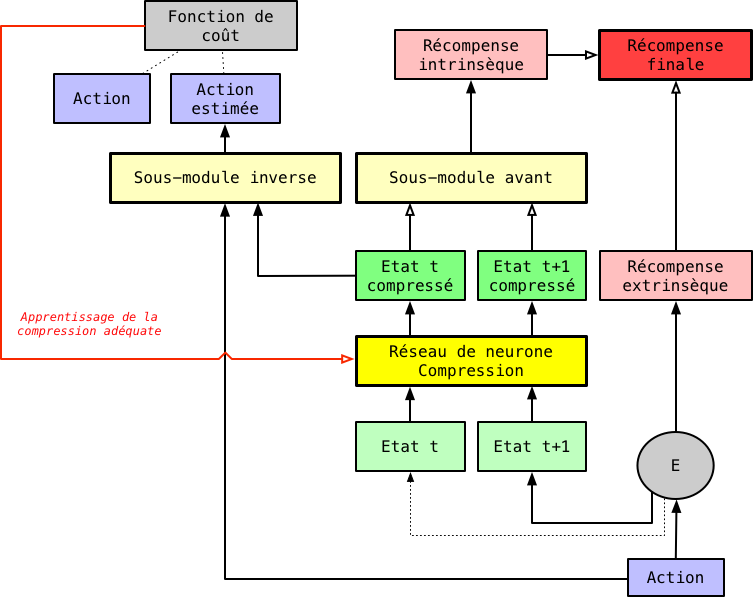
\includegraphics[scale=.4]{./assets/CURIOSITY/curiosity2.png}
        \caption{Schéma finale du module de curiosité mise en place}
    \end{center}
\end{figure}

Le module de curiosité est plus complexe que celui présenté ci-dessus néanmoins le module présenté représente l'idée globale de l'algorithme. Ce module de curiosité a été testé conjointenement avec l'A3C-LSTM-GAE avec les environnements Vizdoom (Doom) et SE-STAR. Les premiers résultats sont encourageants mais il faudra rêgler les quelques problèmes d'interface entre SE-STAR et notre contrôleur pour véritable tester la conjonction des deux algorithmes sont des environnements 3D plus complexe sur SE-STAR. 
                          \newpage     

% =================================
% Conclusion
% =================================

\section{Conclusion}                                            \newpage

% =================================
% Glossaire
% =================================

\printnoidxglossary\newpage

% =================================
% Références
% =================================

\bibliographystyle{unsrt}
\bibliography{ref}

% =================================
% DELETE IN THE FUTURE
% just a personal reminder
% =================================

\newpage\newpage

\todo[inline]{The original todo note withouth changed colours.\newline Here's another line.}
\lipsum[11]\unsure{Is this correct?}\unsure{I'm unsure about also!}
\lipsum[11]\change{Change this!}
\lipsum[11]\info{This can help me in chapter seven!}
\lipsum[11]\improvement{This really needs to be improved!\newline\newline What was I thinking?!}
\lipsum[11]
\thiswillnotshow{This is hidden since option `disable' is chosen!}
\improvement[inline]{The following section needs to be rewritten!}
\lipsum[11]

 
% =================================
% Bibliographie
% =================================

\end{document}
